\documentclass[a4paper,12pt]{article}

\usepackage{amsmath,amssymb,bm}
\usepackage{xepersian}
\usepackage{graphicx}
\usepackage{xcolor}
\usepackage{listings}

\definecolor{codebg}{RGB}{245,245,245}
\definecolor{codeframe}{RGB}{200,200,200}
\definecolor{codekeyword}{RGB}{0,0,150}
\definecolor{codestring}{RGB}{150,0,0}
\definecolor{codecomment}{RGB}{0,120,0}

\lstdefinestyle{matlabStyle}{
  language=Matlab,
  backgroundcolor=\color{codebg},
  basicstyle=\latinfont\ttfamily\footnotesize, % مهم: لاتین + مونو
  keywordstyle=\color{codekeyword}\bfseries,
  stringstyle=\color{codestring},
  commentstyle=\color{codecomment}\itshape,
  numberstyle=\tiny\color{gray},
  numbers=left,
  stepnumber=1,
  numbersep=8pt,
  frame=single,
  rulecolor=\color{codeframe},
  breaklines=true,
  breakatwhitespace=true,
  tabsize=4,
  showstringspaces=false,
  captionpos=b
}

\newenvironment{LTRlisting}
  {\begin{latin}\begin{LTR}}
  {\end{LTR}\end{latin}}


\settextfont{XB Niloofar}
\setlatintextfont{Times New Roman}
\setmonofont{Courier New}


\title{استخراج معادلات حرکت آونگ متصل به ارابه}
\author{}
\date{}

\begin{document}

\maketitle

\section{معرفی سیستم}

در این سیستم، یک آونگ ساده به یک ارابه متصل است که می‌تواند در راستای افقی حرکت کند.
مختصات تعمیم‌یافته سیستم به صورت زیر انتخاب می‌شوند:

\[
    q_1 = x
    \qquad , \qquad
    q_2 = \theta
\]

که در آن:

\begin{itemize}
    \item $x$ : مکان افقی ارابه
    \item $\theta$ : زاویه آونگ نسبت به راستای قائم
    \item $M$ : جرم ارابه
    \item $m$ : جرم آونگ
    \item $L$ : طول آونگ
    \item $g$ : شتاب گرانش
\end{itemize}

همچنین دو اصطکاک لزج در نظر گرفته می‌شود:

\begin{itemize}
    \item $b_c$ : ضریب اصطکاک لزج ارابه
    \item $b_p$ : ضریب اصطکاک لزج مفصل آونگ
\end{itemize}

نیروی ورودی افقی اعمال‌شده به ارابه برابر $F$ است.

\begin{figure}[ht!]
    \centering
    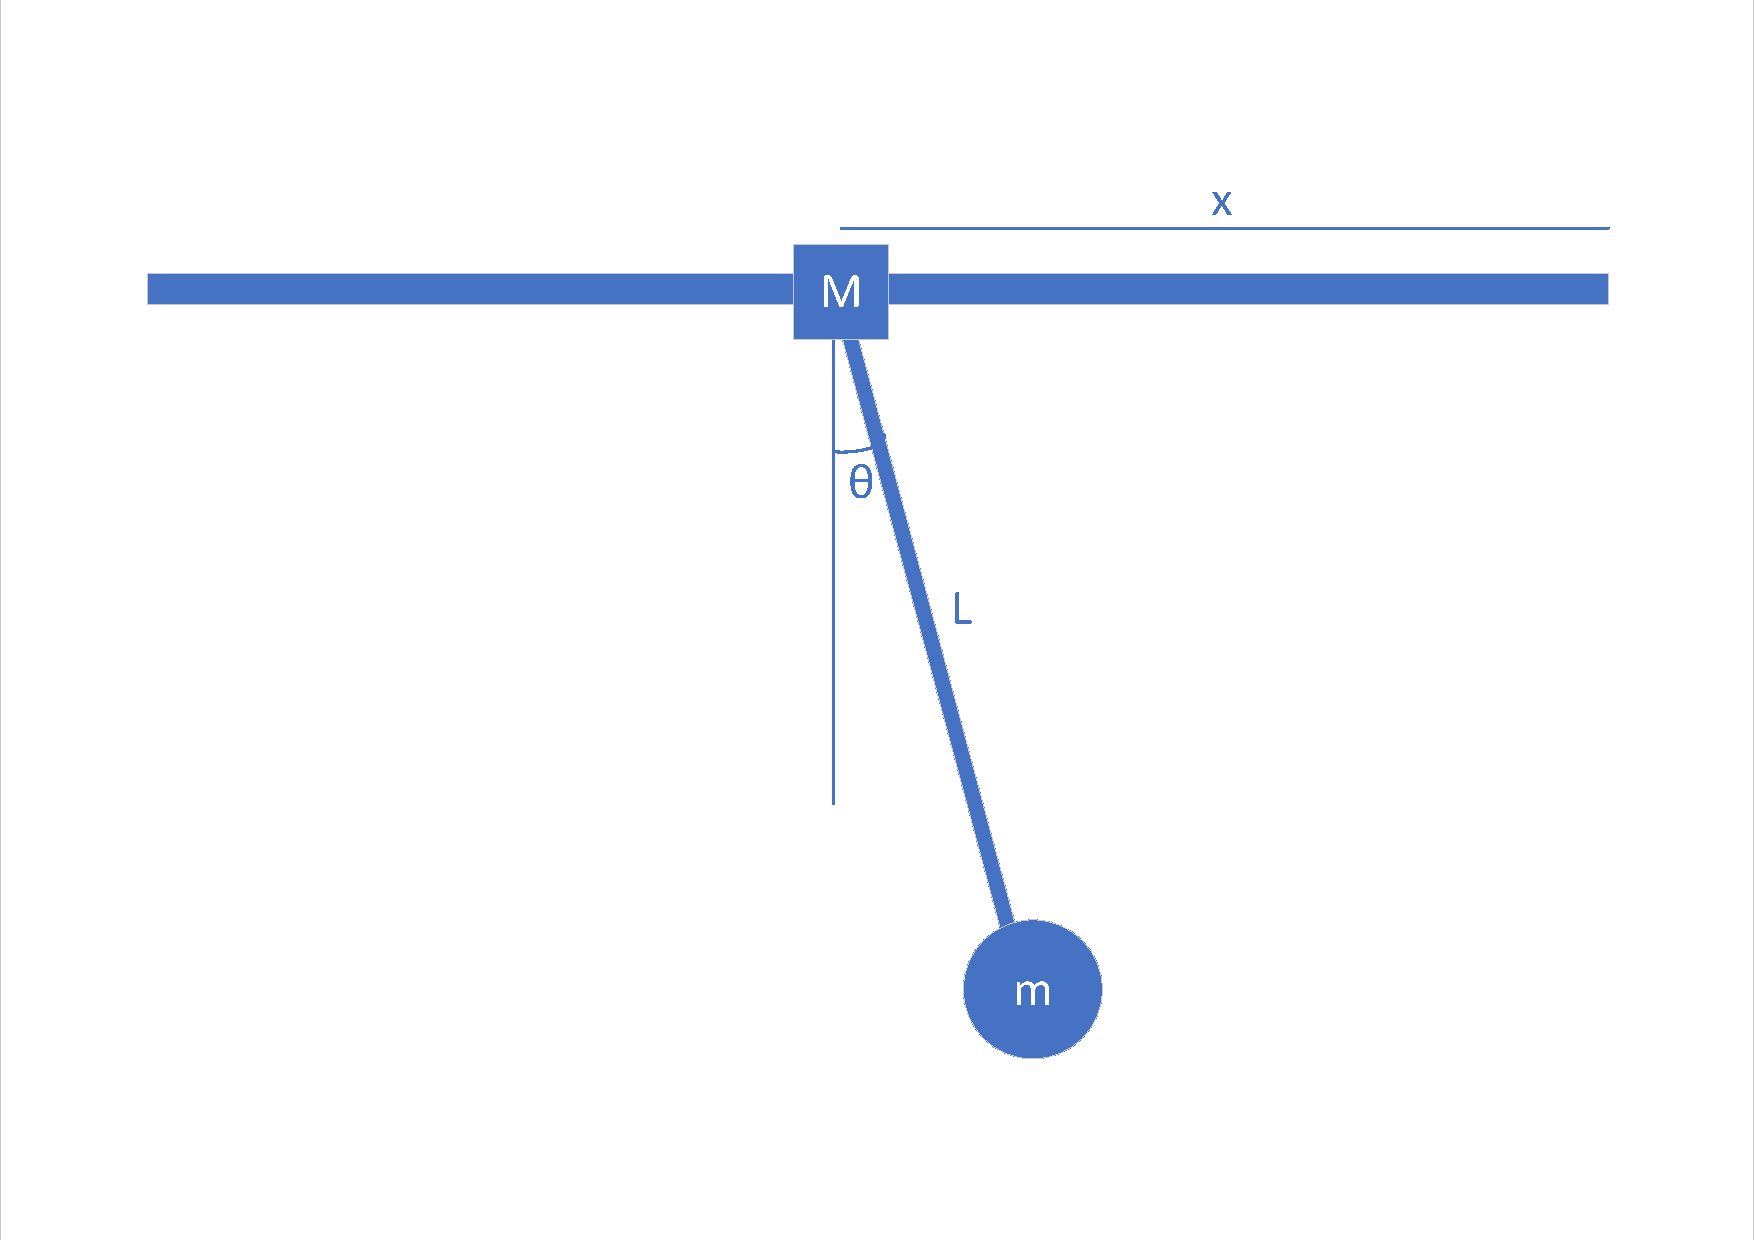
\includegraphics[width=0.7\textwidth]{./images/modeling.pdf}
    \caption{شماتیک سیستم آونگ متصل به ارابه}
    \label{fig:schematic}
\end{figure}


\subsection{مختصات جرم آونگ}

مختصات جرم آونگ برابر است با:

\[
    x_p = x - L \sin\theta
\]

\[
    y_p = -L \cos\theta
\]

با مشتق‌گیری نسبت به زمان:

\[
    \dot{x}_p = \dot{x} - L\dot{\theta}\cos\theta
\]

\[
    \dot{y}_p = L\dot{\theta}\sin\theta
\]

در نتیجه مربع سرعت جرم آونگ:

\[
    v_p^2
    =
    \left(
    \dot{x} - L\dot{\theta}\cos\theta
    \right)^2
    +
    \left(
    L\dot{\theta}\sin\theta
    \right)^2
\]

\subsection{انرژی جنبشی}

انرژی جنبشی ارابه:

\[
    T_c = \frac{1}{2}M\dot{x}^2
\]

انرژی جنبشی جرم آونگ:

\[
    T_p = \frac{1}{2}m v_p^2
\]

بنابراین انرژی جنبشی کل سیستم:

\[
    T
    =
    \frac{1}{2}M\dot{x}^2
    +
    \frac{1}{2}m
    \left[
        \left(
        \dot{x} - L\dot{\theta}\cos\theta
        \right)^2
        +
        \left(
        L\dot{\theta}\sin\theta
        \right)^2
        \right]
\]

با ساده‌سازی:

\[
    T
    =
    \frac{1}{2}(M+m)\dot{x}^2
    -
    mL\dot{x}\dot{\theta}\cos\theta
    +
    \frac{1}{2}mL^2\dot{\theta}^2
\]

\subsection{انرژی پتانسیل}

انرژی پتانسیل گرانشی جرم آونگ برابر است با:

\[
    V = -mgL\cos\theta
\]

\subsection{لاگرانژ سیستم}

تابع لاگرانژ برابر است با:

\[
    \mathcal{L} = T - V
\]

در نتیجه:

\[
    \mathcal{L}
    =
    \frac{1}{2}(M+m)\dot{x}^2
    -
    mL\dot{x}\dot{\theta}\cos\theta
    +
    \frac{1}{2}mL^2\dot{\theta}^2
    +
    mgL\cos\theta
\]

\subsection{نیروهای غیرمحافظه‌کار}

نیروهای اصطکاک لزج به صورت زیر مدل می‌شوند:

\[
    Q_x = F - b_c\dot{x}
\]

\[
    Q_\theta = -b_p\dot{\theta}
\]

\subsection{معادلات اویلر-لاگرانژ}

رابطه کلی اویلر-لاگرانژ:

\[
    \frac{d}{dt}
    \left(
    \frac{\partial \mathcal{L}}
    {\partial \dot{q}_i}
    \right)
    -
    \frac{\partial \mathcal{L}}
    {\partial q_i}
    =
    Q_i
\]

\subsubsection{معادله حرکت ارابه}

برای مختصه $x$:

\[
    \frac{d}{dt}
    \left(
    \frac{\partial \mathcal{L}}
    {\partial \dot{x}}
    \right)
    -
    \frac{\partial \mathcal{L}}
    {\partial x}
    =
    F - b_c\dot{x}
\]

که نتیجه می‌دهد:

\[
    (M+m)\ddot{x}
    -
    mL\ddot{\theta}\cos\theta
    +
    mL\dot{\theta}^2\sin\theta
    =
    F - b_c\dot{x}
\]

\subsection{معادله حرکت آونگ}

برای مختصه $\theta$:

\[
    \frac{d}{dt}
    \left(
    \frac{\partial \mathcal{L}}
    {\partial \dot{\theta}}
    \right)
    -
    \frac{\partial \mathcal{L}}
    {\partial \theta}
    =
    -b_p\dot{\theta}
\]

که در نهایت به رابطه زیر می‌رسیم:

\[
    mL^2\ddot{\theta}
    -
    mL\ddot{x}\cos\theta
    +
    mgL\sin\theta
    =
    -b_p\dot{\theta}
\]

\subsection{معادلات نهایی حرکت}

معادلات دینامیکی سیستم به صورت زیر هستند:

\[
    (M+m)\ddot{x}
    -
    mL\ddot{\theta}\cos\theta
    +
    mL\dot{\theta}^2\sin\theta
    +
    b_c\dot{x}
    =
    F
\]

\[
    mL^2\ddot{\theta}
    -
    mL\ddot{x}\cos\theta
    +
    b_p\dot{\theta}
    +
    mgL\sin\theta
    =
    0
\]

\section{خطی‌سازی و نمایش فضای حالت}

برای طراحی کنترل‌کننده، مدل سیستم حول نقطه تعادل خطی‌سازی می‌شود.
در این مسئله نقطه تعادل متناظر با آونگ آویزان به صورت زیر در نظر گرفته می‌شود:

\[
    \theta \approx 0
\]

با فرض زوایای کوچک، تقریب‌های زیر برقرار هستند:

\[
    \sin\theta \approx \theta
\]

\[
    \cos\theta \approx 1
\]

\[
    \dot{\theta}^2 \approx 0
\]

بنابراین معادلات حرکت خطی‌شده به صورت زیر خواهند بود:

\[
    (M+m)\ddot{x}
    -
    mL\ddot{\theta}
    +
    b_c\dot{x}
    =
    F
\]

\[
    mL^2\ddot{\theta}
    -
    mL\ddot{x}
    +
    b_p\dot{\theta}
    +
    mgL\theta
    =
    0
\]

\subsection{استخراج شتاب‌ها}

از معادله دوم داریم:

\[
    mL^2\ddot{\theta}
    =
    mL\ddot{x}
    -
    b_p\dot{\theta}
    -
    mgL\theta
\]

در نتیجه:

\[
    \ddot{\theta}
    =
    \frac{\ddot{x}}{L}
    -
    \frac{b_p}{mL^2}\dot{\theta}
    -
    \frac{g}{L}\theta
\]

این رابطه را در معادله اول قرار می‌دهیم:

\[
    (M+m)\ddot{x}
    -
    mL
    \left(
    \frac{\ddot{x}}{L}
    -
    \frac{b_p}{mL^2}\dot{\theta}
    -
    \frac{g}{L}\theta
    \right)
    +
    b_c\dot{x}
    =
    F
\]

پس از ساده‌سازی:

\[
    M\ddot{x}
    +
    \frac{b_p}{L}\dot{\theta}
    +
    mg\theta
    +
    b_c\dot{x}
    =
    F
\]

در نتیجه:

\[
    \ddot{x}
    =
    \frac{1}{M}
    \left(
    F
    -
    b_c\dot{x}
    -
    \frac{b_p}{L}\dot{\theta}
    -
    mg\theta
    \right)
\]

اکنون با جایگذاری مجدد در رابطه $\ddot{\theta}$:

\[
    \ddot{\theta}
    =
    \frac{1}{ML}
    \left(
    F
    -
    b_c\dot{x}
    -
    \frac{b_p}{L}\dot{\theta}
    -
    mg\theta
    \right)
    -
    \frac{b_p}{mL^2}\dot{\theta}
    -
    \frac{g}{L}\theta
\]

که با ساده‌سازی برابر می‌شود با:

\[
    \ddot{\theta}
    =
    \frac{1}{ML}F
    -
    \frac{b_c}{ML}\dot{x}
    -
    \left(
    \frac{b_p}{ML^2}
    +
    \frac{b_p}{mL^2}
    \right)\dot{\theta}
    -
    \frac{(M+m)g}{ML}\theta
\]

\section{مدل فضای حالت}

بردار حالت به صورت زیر تعریف می‌شود:

\[
    \mathbf{x}
    =
    \begin{bmatrix}
        x_1 \\
        x_2 \\
        x_3 \\
        x_4
    \end{bmatrix}
    =
    \begin{bmatrix}
        x       \\
        \dot{x} \\
        \theta  \\
        \dot{\theta}
    \end{bmatrix}
\]

ورودی سیستم:

\[
    u = F
\]

و بردار خروجی:

\[
    \mathbf{y}
    =
    \begin{bmatrix}
        x \\
        \theta
    \end{bmatrix}
\]

معادلات حالت سیستم برابر خواهند بود با:

\[
    \dot{x}_1 = x_2
\]

\[
    \dot{x}_2
    =
    -\frac{b_c}{M}x_2
    -
    \frac{mg}{M}x_3
    -
    \frac{b_p}{ML}x_4
    +
    \frac{1}{M}u
\]

\[
    \dot{x}_3 = x_4
\]

\[
    \dot{x}_4
    =
    -\frac{b_c}{ML}x_2
    -
    \frac{(M+m)g}{ML}x_3
    -
    \left(
    \frac{b_p}{ML^2}
    +
    \frac{b_p}{mL^2}
    \right)x_4
    +
    \frac{1}{ML}u
\]

در نتیجه فرم ماتریسی فضای حالت به صورت زیر خواهد بود:

\[
    \dot{\mathbf{x}}
    =
    A\mathbf{x}
    +
    B u
\]

\[
    \mathbf{y}
    =
    C\mathbf{x}
    +
    D u
\]

که در آن:

\[
    A =
    \begin{bmatrix}
        0                   & 1                & 0              & 0                \\
        0                   & -\dfrac{b_c}{M}  & -\dfrac{mg}{M} & -\dfrac{b_p}{ML} \\
        0                   & 0                & 0              & 1                \\
        0                   & -\dfrac{b_c}{ML} &
        -\dfrac{(M+m)g}{ML} &
        -\left(
        \dfrac{b_p}{ML^2}
        +
        \dfrac{b_p}{mL^2}
        \right)
    \end{bmatrix}
\]

\[
    B =
    \begin{bmatrix}
        0            \\
        \dfrac{1}{M} \\
        0            \\
        \dfrac{1}{ML}
    \end{bmatrix}
\]

\[
    C =
    \begin{bmatrix}
        1 & 0 & 0 & 0 \\
        0 & 0 & 1 & 0
    \end{bmatrix}
\]

\[
    D =
    \begin{bmatrix}
        0 \\
        0
    \end{bmatrix}
\]

\section{تحلیل حالت--فضا و ویژگی‌های دینامیکی سیستم}
\label{sec:ss_analysis}

در این بخش، مدل خطی‌شده‌ی سیستم آونگ--ارابه در فضای حالت
از دیدگاه‌های مختلف کلاسیک (مقادیر ویژه، توابع انتقال، کنترل‌پذیری و \ldots)
مورد بررسی قرار می‌گیرد.
هدف این تحلیل آن است که
ساختار دینامیکی سیستم، پایداری داخلی و قابلیت کنترل و مشاهده‌ی آن
به صورت دقیق و مبتنی بر تئوری سیستم‌های خطی مشخص شود.

%==========================================================
\subsection{مقادیر ویژه، قطب‌ها و پایداری داخلی}

برای تحلیل پویایی سیستم آونگ–ارابه در فضای حالت، ابتدا ماتریس‌های
\lr{$A,B,C,D$} را بر اساس مدل دینامیکی استخراج کردیم. با در نظر گرفتن
مقادیر عددی زیر برای پارامترهای فیزیکی سیستم:
\begin{align}
    M   & = 1~\mathrm{kg},             &
    m   & = 0.2~\mathrm{kg},           &
    L   & = 0.5~\mathrm{m},              \\
    g   & = 9.81~\mathrm{m/s^2},       &
    b_c & = 0.1~\mathrm{N\,s/m},       &
    b_p & = 0.05~\mathrm{N\,m\,s/rad},
\end{align}
ماتریس حالت $A$ به صورت زیر به دست می‌آید:
\begin{equation}
    A =
    \begin{bmatrix}
        0 & 1    & 0       & 0    \\
        0 & -0.1 & -1.962  & -0.1 \\
        0 & 0    & 0       & 1    \\
        0 & -0.2 & -23.544 & -1.2
    \end{bmatrix}.
\end{equation}

با محاسبه‌ی مقادیر ویژه‌ی ماتریس $A$، نتیجه‌ی زیر حاصل می‌شود:
\begin{equation}
    \lambda(A) =
    \left\{
    0,\;
    -0.0833,\;
    -0.6083 \pm 4.8138\,\mathrm{j}
    \right\}.
\end{equation}

هر یک از این مقادیر ویژه، یک قطب دینامیکی برای سیستم حالت–فضا را نشان می‌دهد و از طریق آن‌ها می‌توان پایداری داخلی سیستم حلقه‌باز را بررسی کرد. تحلیل هر قطب به صورت زیر است:

\begin{itemize}
    \item \textbf{قطب در مبدأ:}
          وجود مقدار ویژه‌ی
          \(
          \lambda_1 = 0
          \)
          نشان می‌دهد که سیستم حلقه‌باز دارای یک \lr{mode} انتگرالی است. این \lr{mode} عمدتاً با مکان ارابه مرتبط است؛ به این معنا که اگر نیرویی به‌طور مقطعی به ارابه وارد شود، مکان آن به صورت انتگرال سرعت تغییر می‌کند و در غیاب کنترل‌کننده تمایل به بازگشت به یک مقدار ثابت از پیش تعیین‌شده ندارد. از دیدگاه پایداری لیاپنوف، حضور قطب در مبدأ منجر به \emph{پایداری مرزی} (نه پایداری مجانبی) می‌شود؛ یعنی برخی پاسخ‌ها کران‌دار هستند، اما به صفر هم همگرا نمی‌شوند.

    \item \textbf{قطب حقیقی منفی:}
          مقدار ویژه‌ی
          \(
          \lambda_2 = -0.0833
          \)
          یک \lr{mode} حقیقی با میراشدگی بسیار کم را توصیف می‌کند. چون قسمت حقیقی آن منفی و کوچک است، متناظر با یک دینامیک بسیار کند و فروکش‌کننده است؛ این \lr{mode} را می‌توان به ترکیبی از حرکت ارابه و آونگ نسبت داد که به تدریج با یک ثابت زمانی تقریباً
          \[
              \tau \approx \frac{1}{|\lambda_2|} \approx 12~\mathrm{s}
          \]
          میرا می‌شود. این رفتار نشان می‌دهد که بخشی از دینامیک سیستم از نظر انرژی ذاتاً کمی میرا است.

    \item \textbf{زوج مختلط مزدوج:}
          دو مقدار ویژه‌ی
          \(
          \lambda_{3,4} = -0.6083 \pm 4.8138\,\mathrm{j}
          \)
          یک \lr{mode} نوسانی میرا را نشان می‌دهند. قسمت حقیقی منفی آن‌ها، میزان میراشدگی و قسمت موهومی آن‌ها، فرکانس نوسان را تعیین می‌کند. فرکانس نوسانی این زوج به صورت زیر قابل محاسبه است:
          \begin{equation}
              \omega_d = 4.8138~\mathrm{rad/s}
              \quad\Rightarrow\quad
              f_d = \frac{\omega_d}{2\pi} \approx 0.77~\mathrm{Hz}.
          \end{equation}
          بنابراین، دینامیک آونگ دارای نوساناتی با فرکانس حدود
          $0.77~\mathrm{Hz}$
          و میراشدگی مشخص (به دلیل اصطکاک‌ها) است. در غیاب کنترل‌کننده، این نوسانات به مرور زمان کاهش می‌یابند، اما این کاهش صرفاً در بخش نوسانی انجام می‌شود و تضمینی برای بازگشت کامل سیستم به مبدأ حالت ($x=0$، $\theta=0$ و غیره) وجود ندارد.
\end{itemize}

\subsubsection*{نتیجه‌گیری درباره پایداری داخلی}

با توجه به این که:
\begin{enumerate}
    \item سه مقدار ویژه دارای قسمت حقیقی منفی هستند
          \(
          (-0.0833,\; -0.6083 \pm 4.8138j)
          \)
          و
    \item یک مقدار ویژه دقیقاً روی مبدأ قرار دارد
          \(
          (\lambda = 0)
          \),
\end{enumerate}
می‌توان نتیجه گرفت که در مدل حلقه‌بازِ مورد بررسی، هیچ \lr{mode} ناپایداری با قسمت حقیقی مثبت وجود ندارد و سه مقدار ویژه دارای قسمت حقیقی منفی هستند. با این حال، حضور یک مقدار ویژه در مبدأ (\(\lambda=0\)) باعث می‌شود که سیستم از دید داخلی تنها \textbf{پایدار مرزی} باشد و \textbf{مجانباً پایدار} نباشد. به بیان دیگر:

\begin{itemize}
    \item پاسخ سیستم در برابر اغتشاشات کوچک واگرا نمی‌شود (سیستم ناپایدار نیست)،
    \item اما تضمینی وجود ندارد که حالت‌ها به مبدأ یا یک حالت تعادلی دلخواه همگرا شوند و به‌ویژه مکان ارابه می‌تواند پس از اعمال ورودی، روی مقادیر ثابتِ غیردلخواه متوقف شود یا حول نقطه‌ی مرجع باقی‌مانده‌هایی داشته باشد.
\end{itemize}

در مسئله‌ی حاضر هدف اصلی این است که ارابه پس از طی مسیر و رسیدن به موقعیت مرجع \(x_d\)، در همان نقطه متوقف شده و نوسانات باقیمانده‌ی آونگ (زاویه و سرعت زاویه‌ای) به حداقل ممکن برسند. رفتار حلقه‌باز سیستم، به دلیل وجود قطب در مبدأ و میراشدگی محدود، به‌تنهایی نمی‌تواند تضمین کند که:

\begin{enumerate}
    \item موقعیت نهایی ارابه دقیقاً برابر \(x_d\) شود،
    \item و نوسانات آونگ پس از رسیدن ارابه به \(x_d\)، به‌طور مؤثر و سریع میرا شوند.
\end{enumerate}

بنابراین، طراحی یک قانون کنترل بازخورد حالت (مثلاً به صورت
\(
u = -Kx + r
\)
با در نظر گرفتن سیگنال مرجع \(r\))
ضروری است تا با انتخاب مناسب ماتریس بهره‌ی \(K\)، قطب‌های سیستم حلقه‌بسته
\(
A_{\text{cl}} = A - BK
\)
در نواحی دلخواه نیم‌صفحه‌ی چپ قرار گیرند. به این ترتیب، می‌توان سرعت میراشدگی دینامیک‌های نوسانی و رفتار گذرای سیستم را به گونه‌ای تنظیم کرد که:

\begin{itemize}
    \item ارابه با خطای ماندگار کوچک به موقعیت \(x_d\) برسد،
    \item و نوسانات باقیمانده‌ی آونگ پس از رسیدن به \(x_d\) تا حد امکان کاهش یافته و سیستم به حالت سکون مطلوب نزدیک شود.
\end{itemize}

در بخش‌های بعدی گزارش، نحوه‌ی طراحی کنترل‌کننده‌ی بازخورد حالت و تأثیر آن بر جابه‌جایی قطب‌های حلقه‌بسته و کاهش نوسانات باقیمانده، به‌صورت عددی و شبیه‌سازی‌شده مورد بررسی قرار خواهد گرفت.

%==========================================================
\subsection{کنترل‌پذیری و پایدارپذیری}
\label{subsec:controllability_stabilizability}

یکی از پرسش‌های اساسی در این پروژه آن است که
با وجود کم‌عملگر بودن سیستم (یک ورودی نیرو برای چهار حالت
$x,\,\dot{x},\,\theta,\,\dot{\theta}$)،
آیا می‌توان با استفاده از فیدبک حالت (به‌ویژه کنترل‌کننده‌ی LQR)
هم‌زمان
\begin{enumerate}
    \item ارابه را به موقعیت مرجع دلخواه $x_d$ رساند و در همان نقطه نگه داشت،
    \item و نوسانات آونگ را در حوالی $x = x_d$ به‌طور مؤثر میرا کرده و به «نوسان صفر» (زاویه و سرعت زاویه‌ای نزدیک به صفر) رساند
\end{enumerate}
یا خیر.
پاسخ این سؤال در چارچوب نظریه‌ی سیستم‌های خطی،
با بررسی \emph{کنترل‌پذیری} و \emph{پایدارپذیری} جفت $(A,B)$ داده می‌شود.

\paragraph{کنترل‌پذیری.}
ماتریس کنترل‌پذیری سیستم به صورت زیر تعریف می‌شود:
\begin{equation}
    \mathcal{C} =
    \big[\, B \;\; A B \;\; A^2 B \;\; A^3 B \,\big]
    \in \mathbb{R}^{4\times 4}.
\end{equation}
اگر رتبه‌ی این ماتریس برابر با بعد فضای حالت باشد، یعنی
\begin{equation}
    \mathrm{rank}(\mathcal{C}) = 4,
\end{equation}
آنگاه جفت $(A,B)$ \emph{کاملاً کنترل‌پذیر} است.
در این حالت، می‌توان با انتخاب بهره‌ی مناسب $K$ در قانون فیدبک حالت
\[
    u = -Kx + r,
\]
قطب‌های سیستم حلقه‌بسته
\(
A_{\mathrm{cl}} = A - BK
\)
را (پس از خطی‌سازی حول نقطه‌ی کار مناسب) به نواحی دلخواه نیم‌صفحه‌ی چپ منتقل کرد و سرعت میراشدگی و شکل پاسخ گذرا را مطابق نیاز تنظیم نمود.

در این پروژه، با استفاده از نرم‌افزار متلب و دستورهای
\texttt{ctrb} و \texttt{rank}،
ماتریس کنترل‌پذیری تشکیل و رتبه‌ی آن محاسبه شده است.
نتیجه نشان می‌دهد که:
\[
    \mathrm{rank}(\mathcal{C}) = 4,
\]
بنابراین سیستم آونگ–ارابه با آونگ آویزان
\emph{علی‌رغم کم‌عملگر بودن، از دیدگاه خطی کاملاً کنترل‌پذیر است}.
این نتیجه از دو جهت برای هدف پروژه کلیدی است:
\begin{itemize}
    \item از دیدگاه داخلی، می‌توان با انتخاب $K$، تمامی مودهای دینامیکی (شامل مود انتگرالی $\lambda_1=0$، مود حقیقی کند و مود نوسانی میرا) را جابه‌جا و میرا کرد؛ در نتیجه، رسیدن به نوسان بسیار کوچک آونگ در حوالی $x = x_d$ از لحاظ تئوری امکان‌پذیر است.
    \item از دیدگاه طراحی عملی، این کنترل‌پذیری کامل مبنای نظری لازم برای اعمال روش‌های بهینه‌سازی مانند LQR را فراهم می‌کند تا بتوان به‌طور سیستماتیک بین دقت در دنبال‌کردن $x_d$ و کاهش نوسانات $\theta$ و $\dot{\theta}$ مصالحه‌ی مناسبی برقرار کرد.
\end{itemize}

\paragraph{پایدارپذیری.}
در حالت کلی، ممکن است سیستم به طور کامل کنترل‌پذیر نباشد؛
اما تا زمانی که همه‌ی مودهای ناپایدار کنترل‌پذیر باشند،
سیستم را \emph{پایدارپذیر} (\lr{stabilizable}) می‌نامند.
به بیان دقیق‌تر، اگر هر مقدار ویژه‌ی $A$ که قسمت حقیقی مثبت دارد
در زیرفضای کنترل‌پذیر قرار گیرد،
می‌توان با فیدبک حالت مناسب، این مودهای ناپایدار را پایدار نمود
و مودهای پایدارِ غیرقابل کنترل را بدون ایجاد مشکل رها کرد.

در سیستم حاضر، طیف مقادیر ویژه‌ی حلقه‌باز
\[
    \lambda(A) =
    \left\{
    0,\;
    -0.0833,\;
    -0.6083 \pm 4.8138\,\mathrm{j}
    \right\}
\]
نشان می‌دهد که سیستم فاقد مود با قسمت حقیقی مثبت است و تنها از دید داخلی \emph{پایدار مرزی} است (به‌دلیل وجود قطب در مبدأ).
از سوی دیگر، با توجه به این‌که $(A,B)$ کاملاً کنترل‌پذیر است،
پایدارپذیری نیز به‌طور خودکار برقرار می‌شود.
این بدین معناست که:
\begin{itemize}
    \item می‌توان با فیدبک حالت مناسب، مود انتگرالی مرتبط با $\lambda = 0$ را نیز به نیم‌صفحه‌ی چپ منتقل کرد و از پایداری مرزی به پایداری مجانبی گذر نمود،
    \item و در عین حال، مودهای نوسانی مرتبط با حرکت آونگ را با انتخاب $K$ (یا به‌صورت معادل با انتخاب وزن‌های $Q$ و $R$ در LQR) به اندازه‌ی کافی میرا کرد تا نوسانات باقیمانده پس از رسیدن ارابه به $x_d$ به حداقل برسند.
\end{itemize}

در مجموع، کنترل‌پذیری کامل و پایدارپذیری جفت $(A,B)$ تضمین می‌کند که
\textbf{از منظر تئوری، طراحی یک کنترل‌کننده‌ی LQR که ارابه را در $x = x_d$ نگه داشته و نوسان آونگ را به‌طور مؤثر میرا کند (تقریباً «نوسان صفر» در حالت ماندگار) امکان‌پذیر است}.
در بخش‌های بعدی، نحوه‌ی انتخاب $Q$ و $R$ و نتایج شبیه‌سازی، این نتیجه‌گیری تئوریک را به‌صورت عددی و تجربی تأیید خواهد کرد.

%==========================================================
\subsection{رویت‌پذیری و قابل‌تشخیص‌بودن}
\label{subsec:observability_detectability}

در پیاده‌سازی‌های عملی، معمولاً تنها بخشی از حالات سیستم به‌طور مستقیم قابل اندازه‌گیری هستند.
در این پروژه، مکان ارابه $x$ و زاویه‌ی آونگ $\theta$ به عنوان خروجی اندازه‌گیری می‌شوند
و سرعت‌های $\dot{x}$ و $\dot{\theta}$ باید به کمک یک مشاهده‌گر (observer) تخمین زده شوند.
برای طراحی مشاهده‌گرهایی مانند مشاهده‌گر لونبرگر یا فیلتر کالمن،
بررسی \emph{رویت‌پذیری} جفت $(A,C)$ گام نخست و ضروری است.

\paragraph{رویت‌پذیری.}
ماتریس رویت‌پذیری به صورت زیر تعریف می‌شود:
\begin{equation}
    \mathcal{O} =
    \begin{bmatrix}
        C     \\
        C A   \\
        C A^2 \\
        C A^3
    \end{bmatrix}
    \in \mathbb{R}^{8\times 4}.
\end{equation}
اگر رتبه‌ی این ماتریس برابر با بعد فضای حالت باشد، یعنی
\[
    \mathrm{rank}(\mathcal{O}) = 4,
\]
آنگاه جفت $(A,C)$ \emph{کاملاً رویت‌پذیر} خواهد بود.
در این حالت، می‌توان با استفاده از اندازه‌گیری‌های خروجی $y(t)$
و ورودی اعمالی $u(t)$، حالت کامل $x(t)$ را (در چارچوب مدل خطی)
به‌صورت یکتا و با دقت دلخواه بازسازی کرد.

در این پروژه، با استفاده از دستورهای \texttt{obsv} و \texttt{rank} در متلب،
ابتدا ماتریس رویت‌پذیری $\mathcal{O}$ تشکیل شده و سپس رتبه‌ی آن محاسبه گردیده است.
نتایج عددی نشان می‌دهند که:
\[
    \mathrm{rank}(\mathcal{O}) = 4,
\]
بنابراین جفت $(A,C)$ دارای رویت‌پذیری کامل است
و طراحی مشاهده‌گرهای حالت (از جمله مشاهده‌گر لونبرگر و فیلتر کالمن)
برای این سیستم از نظر تئوری امکان‌پذیر است.

\paragraph{قابل‌تشخیص‌بودن (Detectability).}
به‌طور کلی، حتی اگر سیستم کاملاً رویت‌پذیر نباشد،
در صورتی که تمام مودهای ناپایدار آن رویت‌پذیر باشند،
سیستم را \emph{قابل‌تشخیص (detectable)} می‌نامند.
قابل‌تشخیص‌بودن شرطی کافی برای طراحی مشاهده‌گرهای حالت پایدار است؛
یعنی کافی است تمامی مودهای ناپایدار را بتوان از روی خروجی‌های در دسترس تشخیص داد.

در سیستم آونگ--ارابه‌ی مورد بررسی، با توجه به این‌که جفت $(A,C)$
بر اساس محاسبات متلب کاملاً رویت‌پذیر است،
شرط قابل‌تشخیص‌بودن نیز به‌طور خودکار برقرار خواهد بود.
در نتیجه، در کنار کنترل‌پذیری کامل سیستم، امکان طراحی مشاهده‌گرهای پایدار نیز تضمین می‌شود
و می‌توان در مراحل بعدی، ساختار \emph{کنترل‌کننده--مشاهده‌گر} (برای مثال LQG)
را برای پیاده‌سازی عملی مد نظر قرار داد.

%==========================================================
\subsection{جمع‌بندی تحلیل حالت--فضا}

نتایج تحلیل حالت--فضا در این پروژه را می‌توان به صورت خلاصه به شکل زیر بیان کرد:
\begin{itemize}
    \item مقادیر ویژه‌ی ماتریس $A$ ساختار دینامیکی ذاتی سیستم را تعیین می‌کنند
          و نشان می‌دهند که مدل خطی‌شده‌ی سیستم آونگ--ارابه
          در حالت حلقه‌باز دارای یک مود انتگرالی و یک جفت مود نوسانی میرا است.
          با انتخاب مناسب فیدبک حالت (برای مثال از طریق LQR)،
          می‌توان تمامی این مقادیر ویژه را به نیم‌صفحه‌ی چپ منتقل کرد
          و پایداری داخلی سیستم را در اطراف نقطه‌ی کار تضمین نمود.
    \item ماتریس کنترل‌پذیری جفت $(A,B)$ دارای رتبه‌ی کامل است؛
          بنابراین، علی‌رغم کم‌عملگر بودن (یک ورودی برای چهار حالت)،
          سیستم از دیدگاه خطی \emph{کاملاً کنترل‌پذیر و پایدارپذیر} است
          و طراحی یک کنترل‌کننده‌ی LQR برای پایدارسازی موضعی تعادل مورد نظر
          و میرایش نوسانات آونگ، از نظر تئوری امکان‌پذیر می‌باشد.
    \item ماتریس رویت‌پذیری جفت $(A,C)$، نیز دارای رتبه‌ی کامل است؛
          در نتیجه، سیستم \emph{کاملاً رویت‌پذیر و قابل‌تشخیص} است حتی در حالتی که تنها مکان ارابه و زاویه پاندول اندازه‌گیری می‌شود.
          این ویژگی اجازه می‌دهد که از مشاهده‌گرهای حالت (مانند مشاهده‌گر لونبرگر
          یا فیلتر کالمن) برای تخمین حالات غیرقابل اندازه‌گیری
          استفاده شود.
\end{itemize}

\section{طراحی، شبیه‌سازی و پیاده‌سازی کنترل‌کننده بهینه \lr{LQR}}
\label{sec:lqr_design}

با توجه به اثبات کنترل‌پذیری کامل سیستم در بخش‌های پیشین، در این بخش از کنترل‌کننده بهینه خطی تنظیم‌کننده مربعی یا \lr{LQR (Linear Quadratic Regulator)} برای پایدارسازی موقعیت ارابه و میرایش نوسانات آونگ استفاده می‌شود. هدف این کنترل‌کننده، یافتن ماتریس بهره بهینه فیدبک حالت $K$ در قانون کنترل $u = -K\mathbf{x}$ است به گونه‌ای که تابع هزینه مربعی زیر کمینه شود:

\begin{equation}
    J = \int_{0}^{\infty} \left( \mathbf{x}^T Q \mathbf{x} + u^T R u \right) dt
\end{equation}

که در آن $Q \in \mathbb{R}^{4 \times 4}$ ماتریس وزن‌دهی به خطای متغیرهای حالت و $R > 0$ اسکالر معین مثبت برای وزن‌دهی به تلاش کنترلی (نیروی اعمالی $F$) است.

\subsection{تنظیم ماتریس‌های وزن‌دهی و محاسبه ماتریس بهره ($K$)}

سیستم مورد بررسی یک آونگ آویزان است؛ بنابراین اهداف عملکردی کنترل‌کننده عبارتند از: رساندن ارابه به موقعیت مرجع بدون فراجهش نامطلوب (\lr{Overshoot}) و کمینه کردن نوسانات زاویه‌ای آونگ (\lr{Anti-sway}). پس از بررسی رفتار سیستم و طی کردن فرآیند تنظیم پارامترها (\lr{Tuning})، ماتریس‌های وزن‌دهی به صورت قطری زیر انتخاب شدند:

\begin{equation}
    Q =
    \begin{bmatrix}
        100 & 0  & 0   & 0  \\
        0   & 50 & 0   & 0  \\
        0   & 0  & 500 & 0  \\
        0   & 0  & 0   & 50
    \end{bmatrix}
    \qquad , \qquad
    R = 1
\end{equation}

منطق فیزیکی حاکم بر انتخاب این ضرایب به شرح زیر است:
\begin{itemize}
    \item $q_1 = 100$: جریمه خطای موقعیت ارابه ($x$) جهت تضمین بازگشت دقیق و سریع به مبدأ تعادل.
    \item $q_2 = 50$: جریمه سرعت ارابه ($\dot{x}$) که به عنوان یک ترمز مجازی یا میرایی فیزیکی عمل می‌کند. بالا بودن این ضریب سبب می‌شود ارابه پیش از رسیدن به نقطه هدف سرعت خود را کم کند تا از ایجاد فراجهش جلوگیری شود.
    \item $q_3 = 500$: اختصاص بیشترین وزن به خطای زاویه آونگ ($\theta$). از آنجا که حذف نوسانات پاندول در کاربردهای صنعتی (مانند جرثقیل‌ها) اولویت اصلی ایمنی است، این ضریب کنترل‌کننده را مجبور می‌کند تا بیشترین تلاش خود را معطوف به قائم نگه داشتن آونگ کند.
    \item $q_4 = 50$: وزن سرعت زاویه‌ای آونگ ($\dot{\theta}$) جهت فروکش کردن سریع نوسانات باقیمانده.
    \item $R = 1$: جریمه تلاش کنترلی به صورت پایه در نظر گرفته شده تا عملگر آزادی عمل کافی برای اعمال نیروی لازم را داشته باشد.
\end{itemize}

با حل معادله جبری ریکاتی پیوسته (\lr{CARE}) به کمک دستور \texttt{lqr} در نرم‌افزار متلب، بردار بهره بهینه فیدبک حالت به صورت دقیق زیر حاصل شد:
\begin{equation}
    K = \begin{bmatrix} 10.0000 & 9.2843 & 26.5142 & 4.1460 \end{bmatrix}
\end{equation}

بنابراین، قانون فیدبک حالت نهایی که به سیستم اعمال می‌شود برابر است با:
\begin{equation}
    F = -(10.0000 x + 9.2843 \dot{x} + 26.5142 \theta + 4.1460 \dot{\theta})
\end{equation}

%======================================================================
\subsection{ارزیابی عملکرد بر روی مدل خطی‌شده سیستم (کد متلب)}

در گام نخست، عملکرد کنترل‌کننده بر روی مدل فضای حالت خطی‌شده سیستم (که در بخش‌های قبلی استخراج شد) به ازای شرایط اولیه اغتشاشی زیر شبیه‌سازی گردید:
\[
    x_0 = 0.5~\mathrm{m}, \quad \dot{x}_0 = 0~\mathrm{m/s}, \quad \theta_0 = 0.2~\mathrm{rad}, \quad \dot{\theta}_0 = 0~\mathrm{rad/s}
\]

شکل \ref{fig:linear_response} پاسخ زمانی متغیرهای حالت سیستم خطی و شکل \ref{fig:linear_effort} سیگنال تلاش کنترلی (نیروی $F$) مربوط به آن را نشان می‌دهند.

\begin{figure}[ht!]
    \centering
    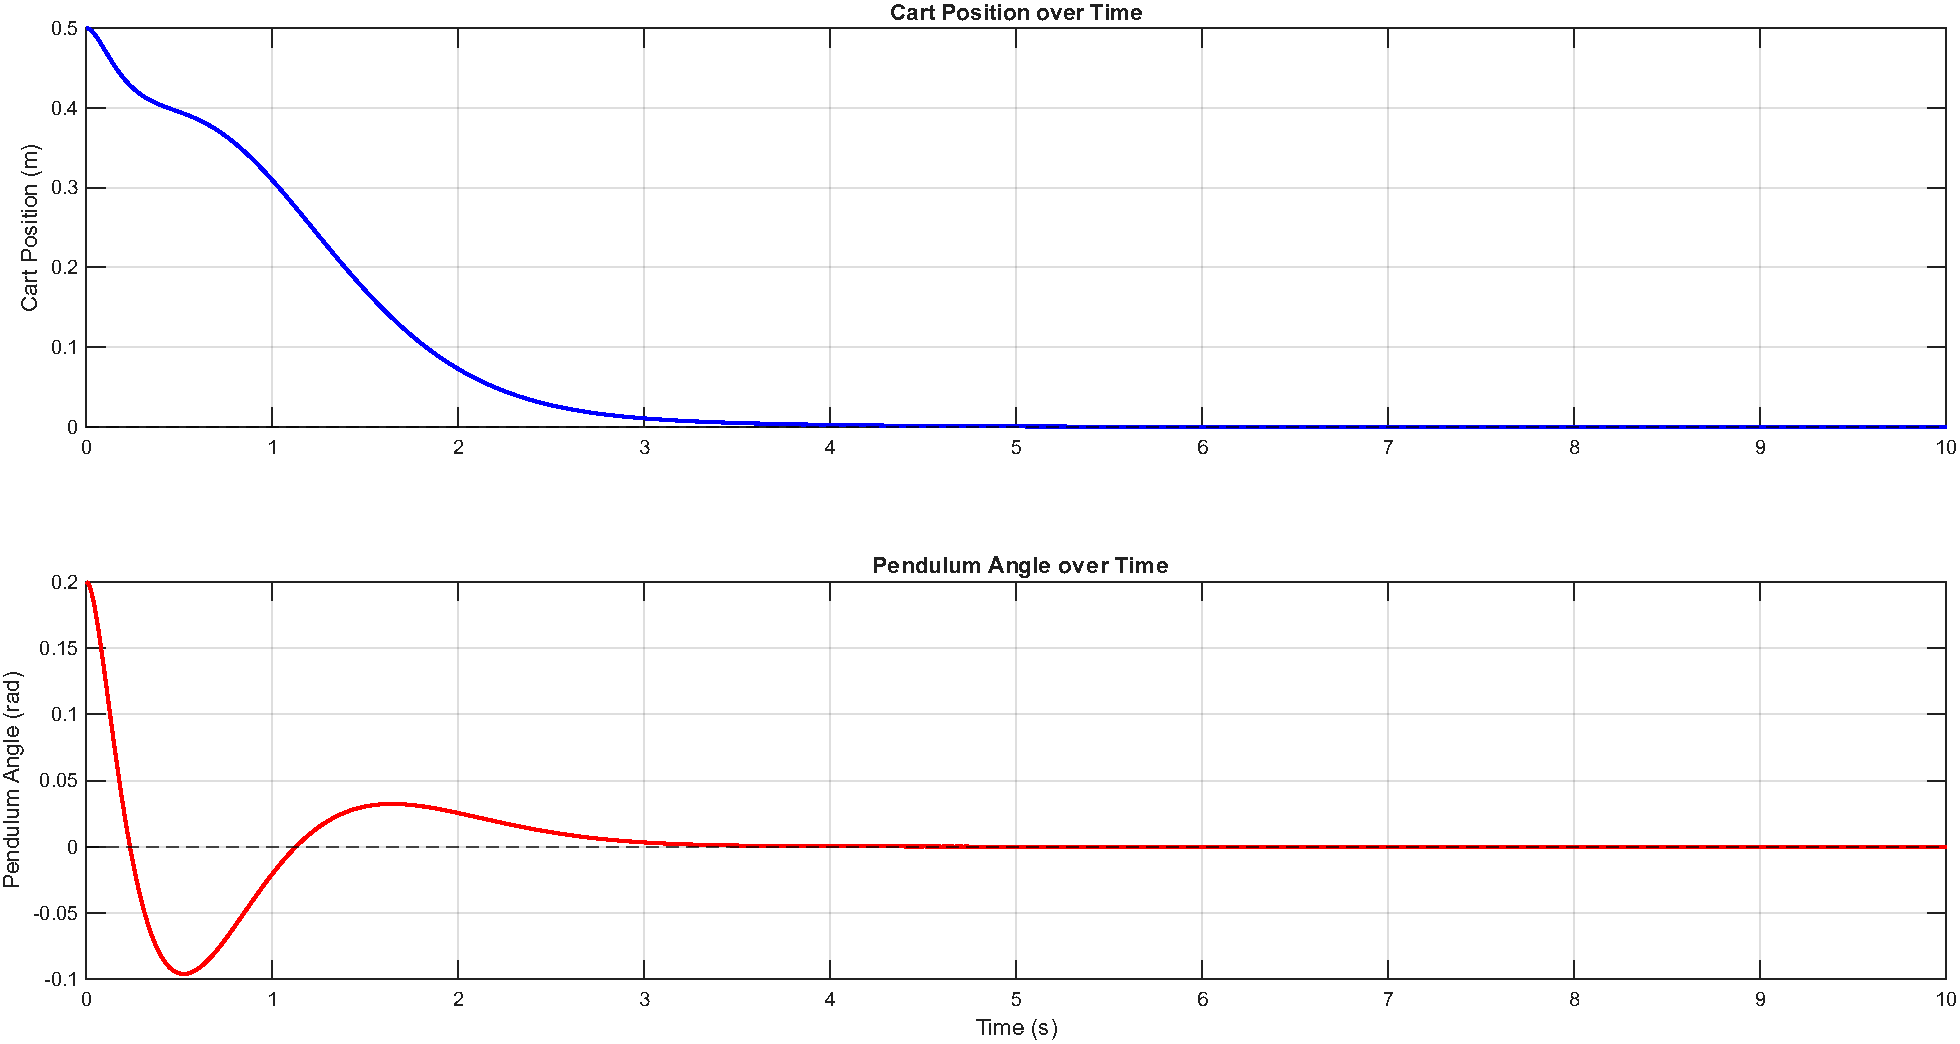
\includegraphics[width=0.8\textwidth]{./images/LQR Initial Condition Response.pdf}
    \caption{پاسخ زمانی متغیرهای حالت (موقعیت ارابه و زاویه آونگ) در مدل خطی‌شده سیستم}
    \label{fig:linear_response}
\end{figure}

\begin{figure}[ht!]
    \centering
    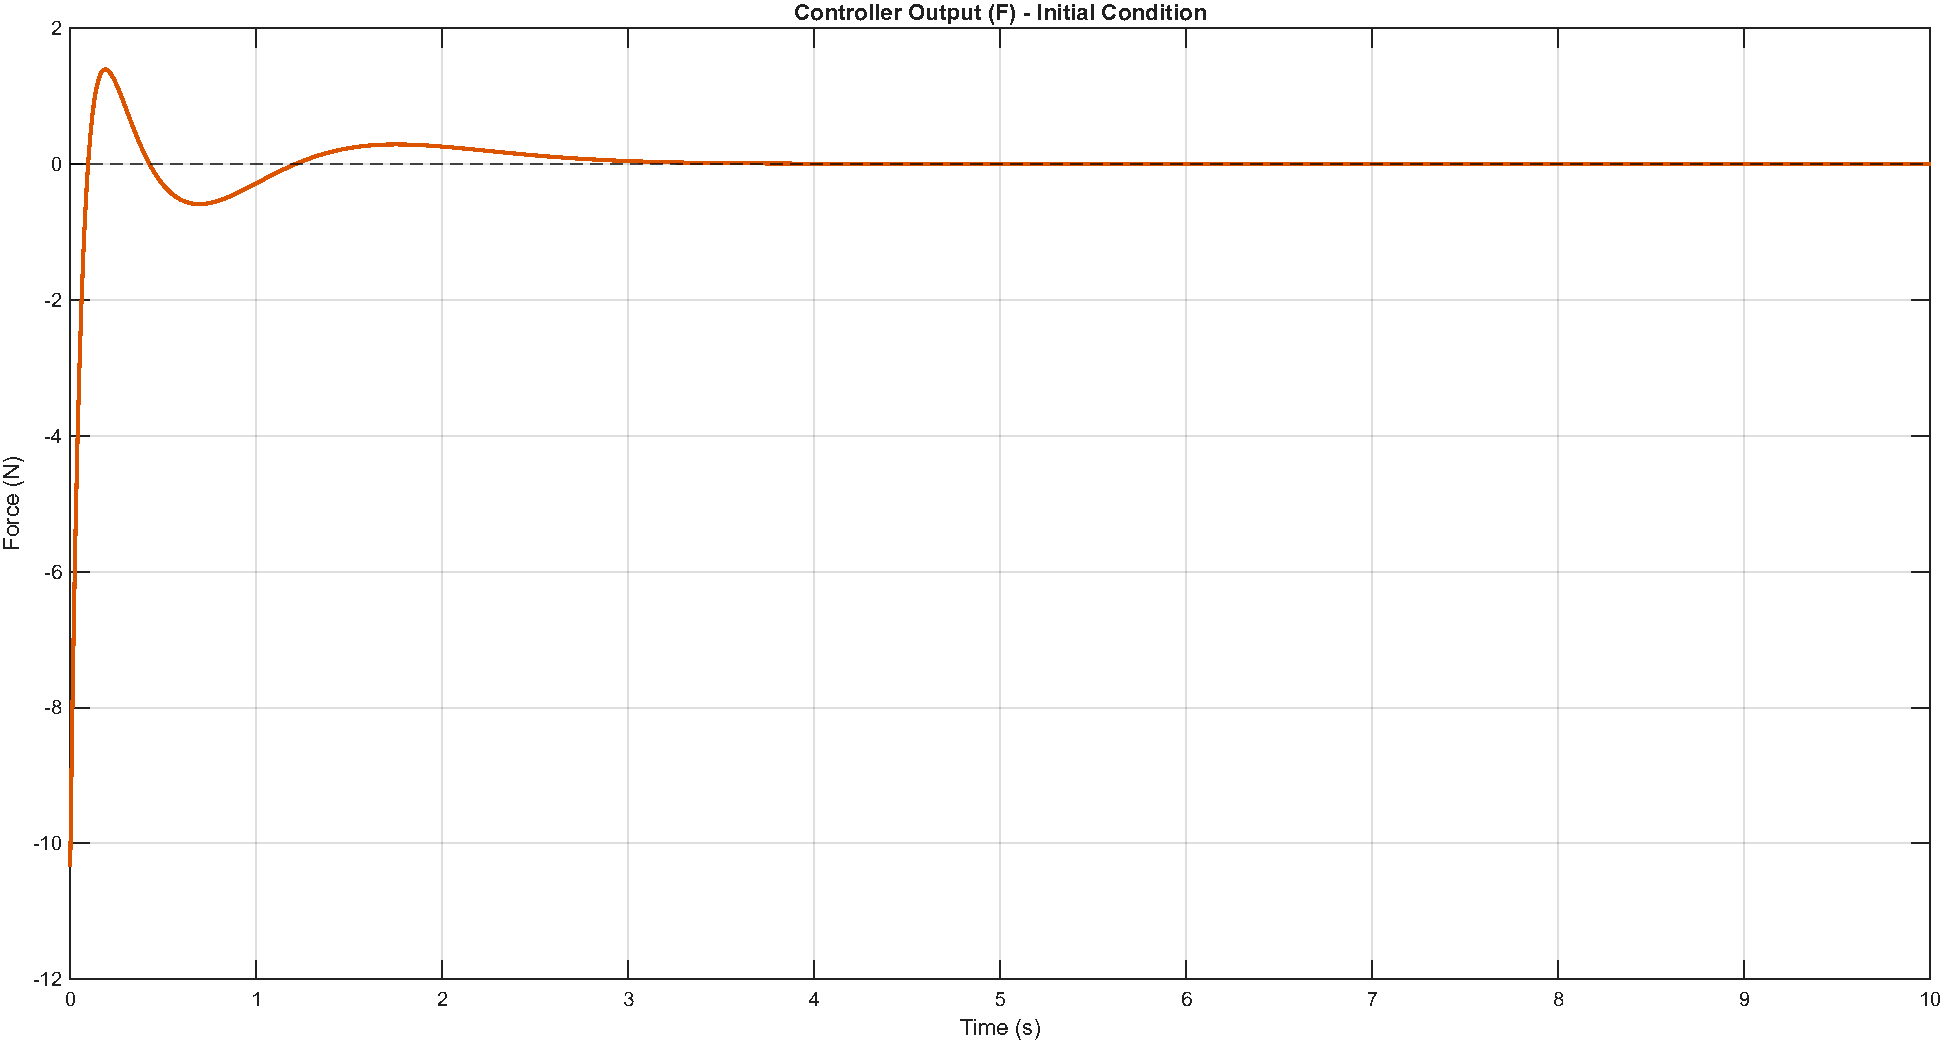
\includegraphics[width=0.8\textwidth]{./images/Control Effort (Initial Condition).pdf}
    \caption{سیگنال تلاش کنترلی (نیروی اعمالی به ارابه) در مدل خطی‌شده سیستم}
    \label{fig:linear_effort}
\end{figure}

مطابق نمودارهای سیستم خطی، مشاهده می‌شود که مکان ارابه به صورت کاملاً اکیداً یکنواخت و بدون هیچ‌گونه فراجهشی به مبدأ بازگشته است که صحت تنظیم ضریب $q_2 = 50$ را تایید می‌کند. نوسانات زاویه‌ای آونگ نیز به دلیل وزن بالای $q_3 = 500$ ظرف مدت کمتر از ۳ ثانیه کاملاً میرا شده‌اند. بیشینه نیروی درخواستی کنترل‌کننده خطی در لحظه اول حدود $10.3~\mathrm{N}$ است که رفتاری کاملاً هموار دارد.

%======================================================================
\subsection{پیاده‌سازی در محیط \lr{Simscape} و ارزیابی روی مدل غیرخطی}

از آنجا که مدل‌های خطی‌شده تنها رفتار سیستم را در همسایگی کوچک نقطه کار تقریب می‌زنند، صحت‌سنجی عملکرد کنترل‌کننده روی دینامیک واقعی و غیرخطی سیستم امری ضروری است. بدین منظور، مدل فیزیکی مکانیزم آونگ--ارابه با در نظر گرفتن تمامی عبارات غیرخطی مثلثاتی و جفت‌شدگی‌های دینامیکی کامل در محیط \lr{Simscape} نرم‌افزار سیمولینک (فایل \texttt{main.slx}) پیاده‌سازی شد.

ساختار فیدبک کامل حالت (\lr{Full State Feedback}) در این محیط پیاده‌سازی گردیده است؛ بدین صورت که خروجی‌های موقعیت ارابه ($x$) و زاویه آونگ ($\theta$) از سنسورهای فیزیکی دریافت شده و با استفاده از بلوک‌های مشتق‌گیر ایده‌آل، سرعت خطی ($\dot{x}$) و سرعت زاویه‌ای ($\dot{\theta}$) استخراج می‌شوند. سپس این ۴ سیگنال بر اساس ترتیب بردار حالت در بلوک \lr{Mux} چیدمان شده و پس از ضرب در ماتریس بهره $-K$، به عنوان نیروی محرک به مکانیسم اعمال می‌گردند (شکل \ref{fig:simscape_block}).

\begin{figure}[ht!]
    \centering
    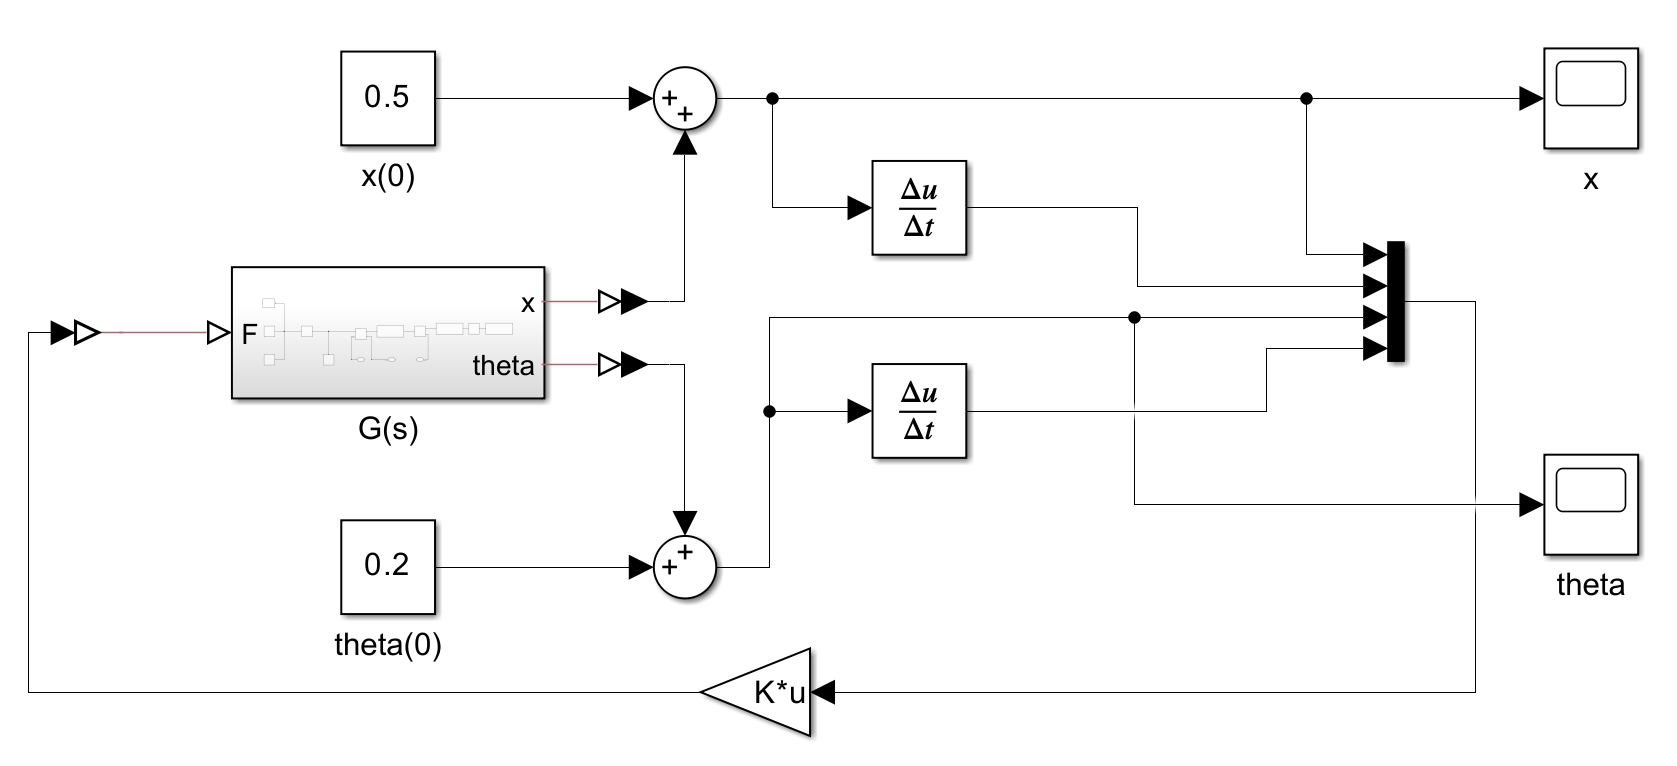
\includegraphics[width=0.9\textwidth]{./images/simscape.png}
    \caption{بلاک دیاگرام پیاده‌سازی سیستم آونگ--ارابه و حلقه فیدبک حالت \lr{LQR} در محیط \lr{Simscape}}
    \label{fig:simscape_block}
\end{figure}

شبیه‌سازی مدل غیرخطی \lr{Simscape} دقیقاً تحت همان شرایط اولیه قبلی ($x_0=0.5$ و $\theta_0=0.2$) اجرا شد. نتایج پاسخ زمانی متغیرها و تلاش کنترلی در شکل‌های \ref{fig:simscape_response} و \ref{fig:simscape_effort} نشان داده شده است.

\begin{figure}[ht!]
    \centering
    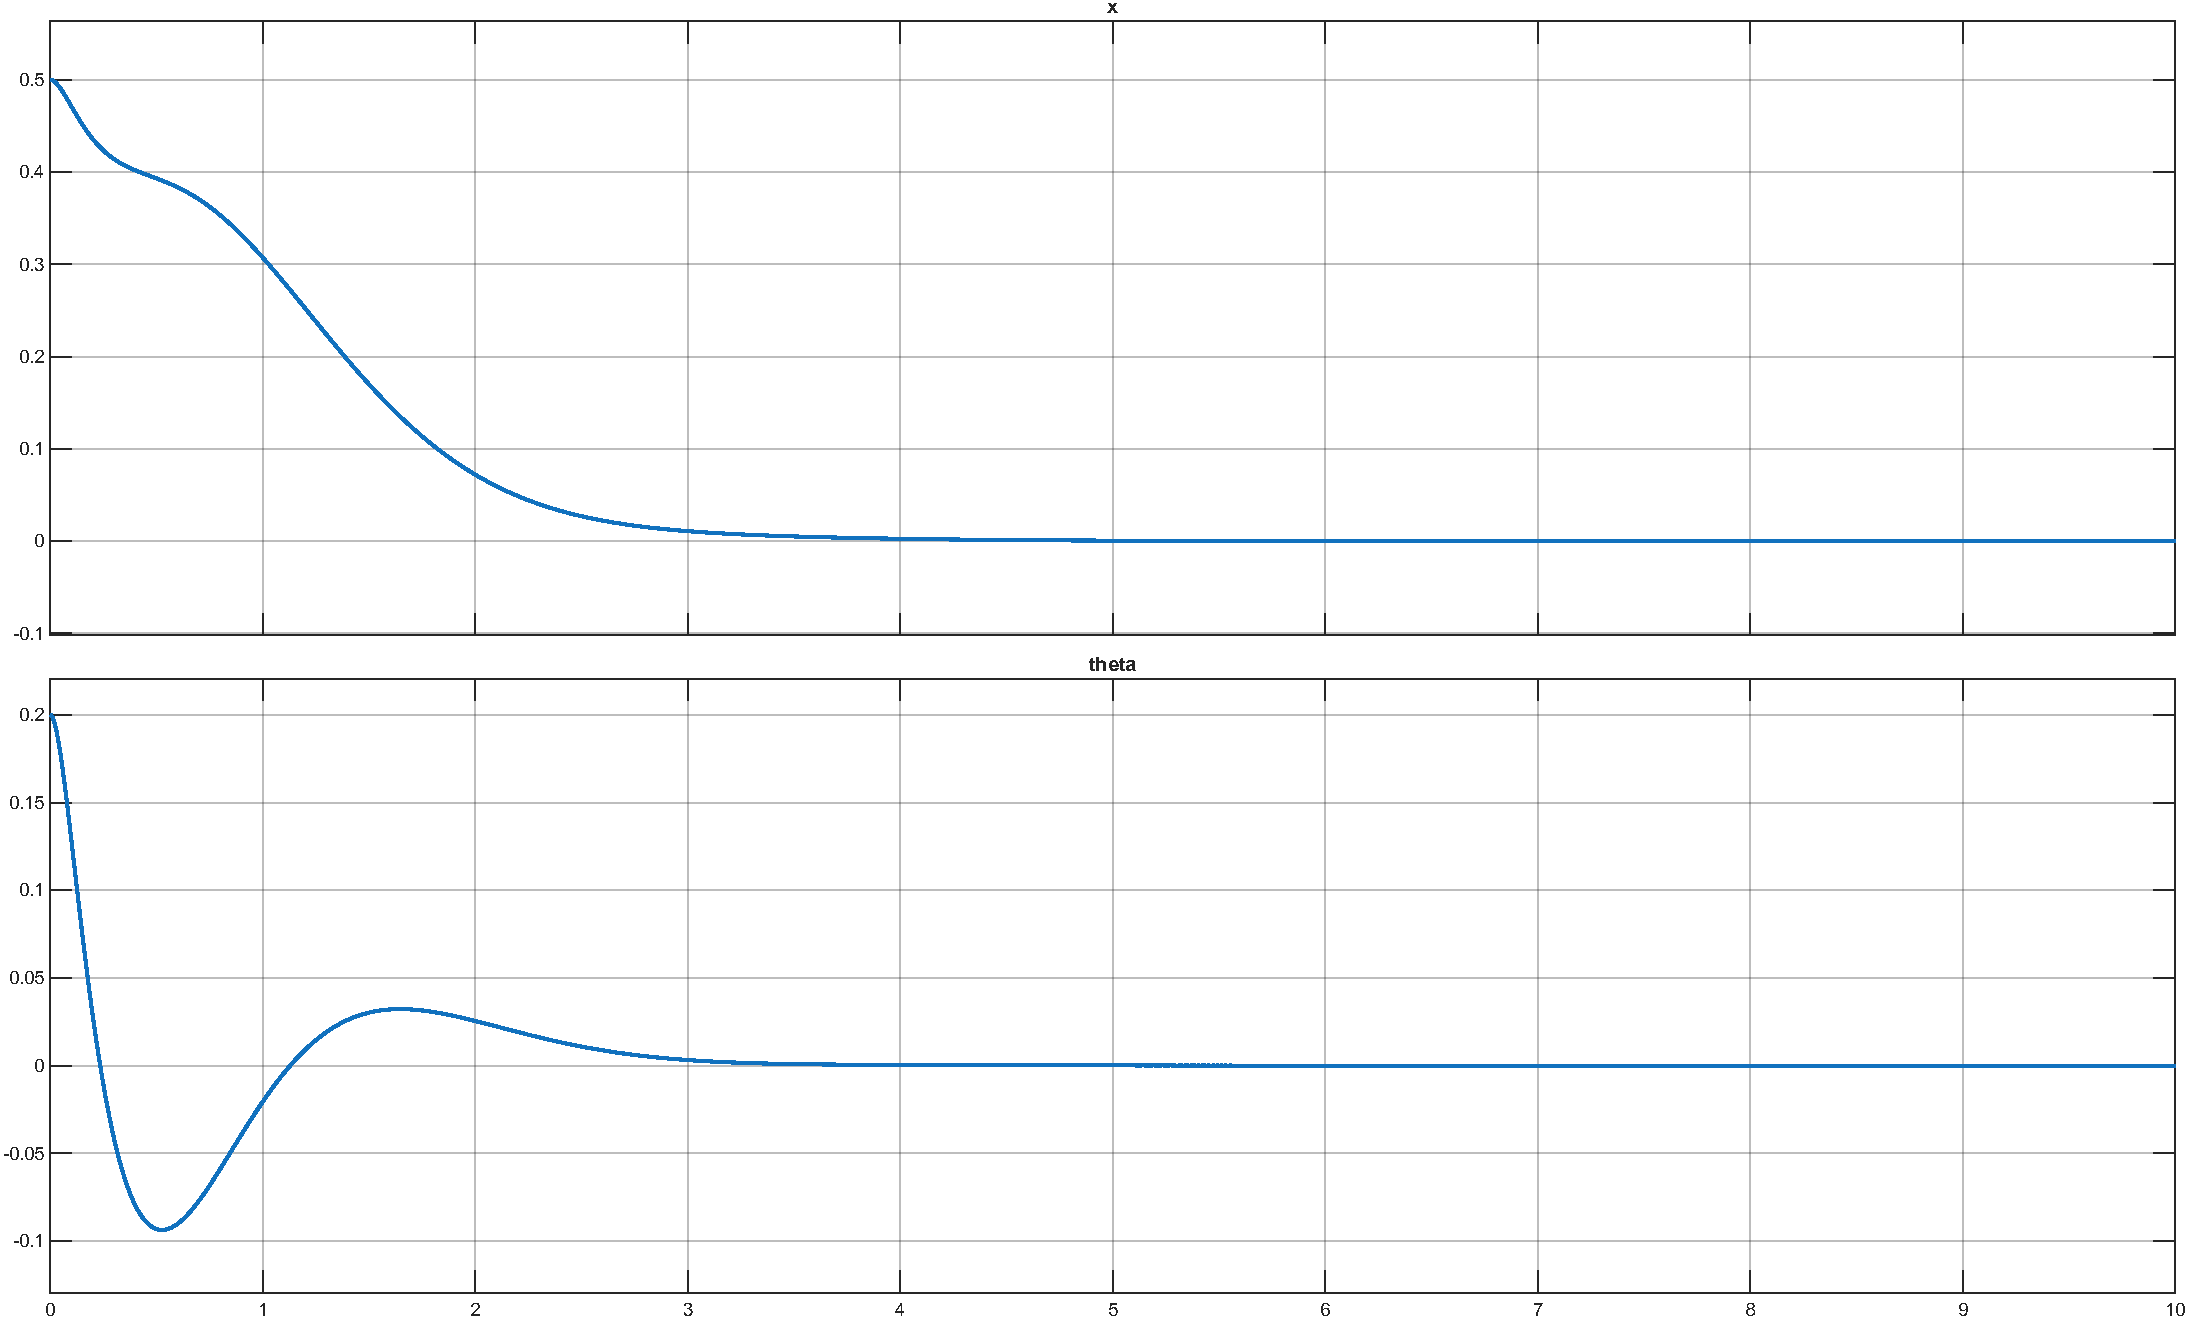
\includegraphics[width=0.8\textwidth]{./images/Simscape Initial Condition Response.pdf}
    \caption{پاسخ زمانی متغیرهای حالت به شرایط اولیه در مدل غیرخطی \lr{Simscape}}
    \label{fig:simscape_response}
\end{figure}

\begin{figure}[ht!]
    \centering
    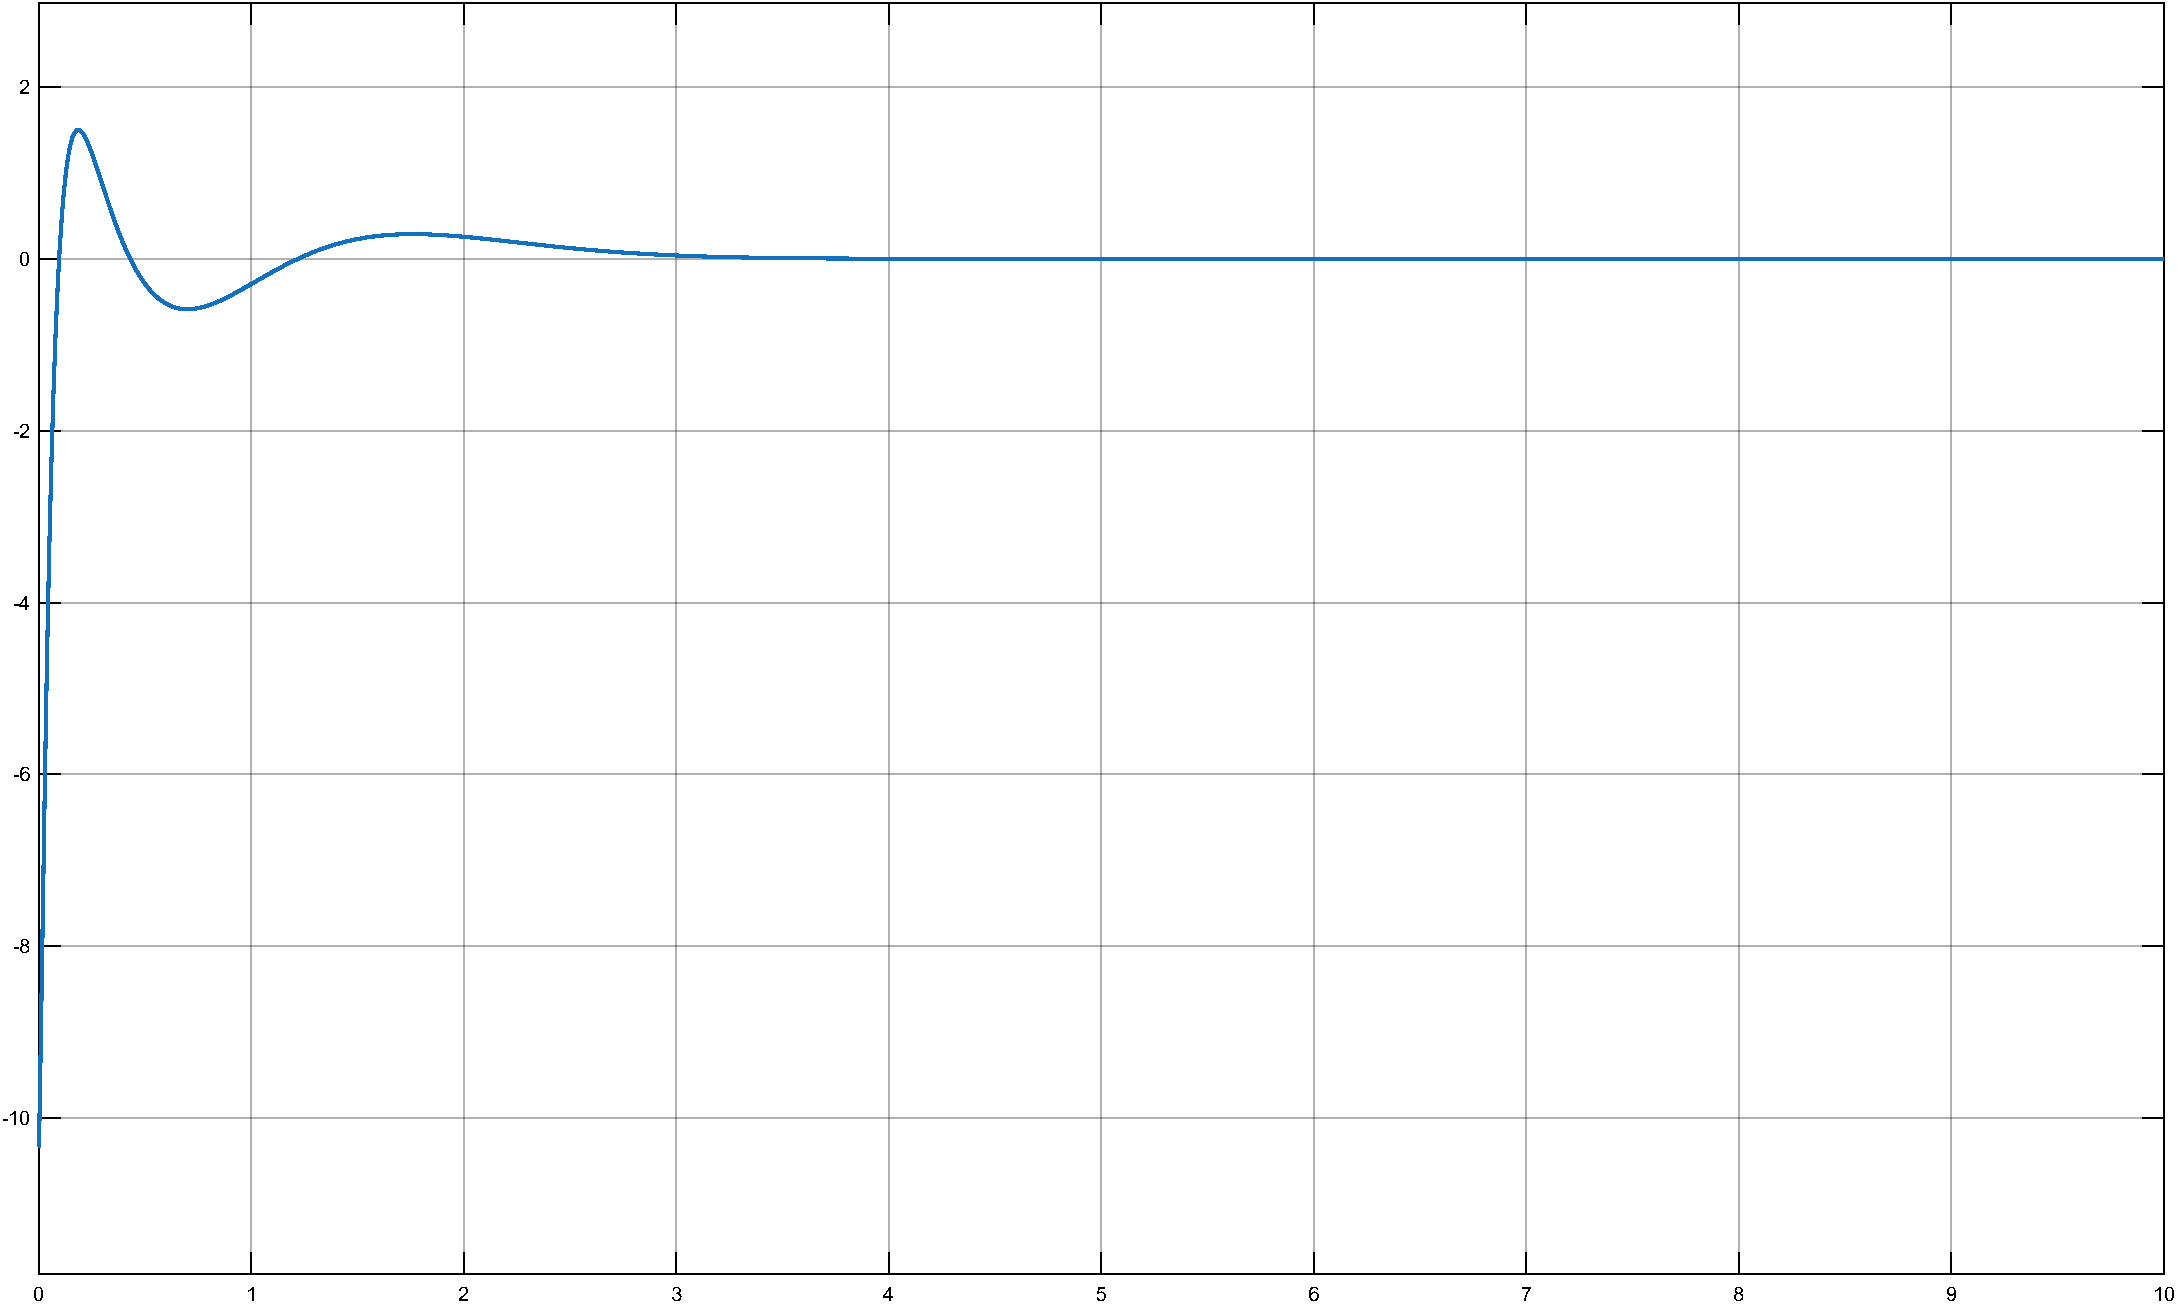
\includegraphics[width=0.8\textwidth]{./images/Control Effort (Simscape).pdf}
    \caption{تلاش کنترلی (نیروی اعمالی به ارابه) در مدل غیرخطی \lr{Simscape}}
    \label{fig:simscape_effort}
\end{figure}

\subsection{مقایسه و تحلیل نتایج خطی و غیرخطی}

با مقایسه نمودارهای حاصل از محاسبات فضای حالت خطی (شکل‌های \ref{fig:linear_response} و \ref{fig:linear_effort}) و شبیه‌سازی مکانیکی غیرخطی در \lr{Simscape} (شکل‌های \ref{fig:simscape_response} و \ref{fig:simscape_effort})، نتایج زیر حاصل می‌شود:
\begin{enumerate}
    \item \textbf{پایداری مجانبی و مقاوم بودن:} کنترل‌کننده \lr{LQR} طراحی‌شده بر پایه مدل خطی، پایداری مجانبی مدل غیرخطی را نیز به خوبی تأمین کرده است که نشان‌دهنده پایداری موضعی قوی و مقاوم بودن (\lr{Robustness}) نسبی این کنترل‌کننده بهینه است.
    \item \textbf{انحراف ناچیز رفتار گذرای ناشی از غیرخطی بودن:} در مدل \lr{Simscape}، عبارات مثلثاتی $\sin\theta$ و $\cos\theta$ و همچنین مربع سرعت زاویه‌ای ($\dot{\theta}^2$) به طور کامل شبیه‌سازی شده‌اند. وجود این جملات سبب شده است که پاسخ پاندول در لحظات ابتدایی شبیه‌سازی غیرخطی دارای اندکی فرکانس متفاوت نسبت به مدل خطی باشد، اما ساختار کلی میرایی حفظ شده و سیستم ظرف همان بازه زمانی ۴ ثانیه به سکون کامل رسیده است.
    \item \textbf{انطباق سیگنال نیرو:} رفتار سیگنال نیروی کنترلی در هر دو شبیه‌سازی بسیار به یکدیگر نزدیک است و بیشینه دامنه آن در محدوده مجاز عملگر قرار دارد که از اشباع ناگهانی سیستم جلوگیری می‌کند.
\end{enumerate}

علاوه بر تحلیل‌های فوق، صحت عملکرد و حرکت روان ارابه همراه با میرایش سریع پاندول از طریق انیمیشن سه‌بعدی خروجی واقع‌گرایانه مالتی‌بادی در محیط \lr{Simscape} (ذخیره‌شده در فایل ویدئویی \texttt{simscape.mp4}) به صورت چشمی نیز مورد تایید قرار گرفت.

\section{طراحی مشاهده‌گر حالت بر مبنای فیلتر کالمن و ساختار \lr{LQG}}
\label{sec:kalman_design}

در پیاده‌سازی‌های صنعتی کنترل‌کننده‌های فیدبک حالت، نصب سنسور برای اندازه‌گیری مستقیم تمامی متغیرهای سیستم (به ویژه متغیرهای سرعت و زاویه) معمولاً هزینه‌بر بوده و داده‌های حاصل از آن‌ها به شدت نویزی است. در این بخش از پروژه، فرض واقع‌بینانه‌تری در نظر گرفته شده است: تنها \textbf{موقعیت ارابه ($x$)} توسط یک سنسور (مانند انکودر نوری) اندازه‌گیری می‌شود و سه متغیر دیگر ($\dot{x}, \theta, \dot{\theta}$) باید تخمین زده شوند.

با این فرض، ماتریس خروجی سیستم تنها شامل یک سطر خواهد بود:
\begin{equation}
    C = \begin{bmatrix} 1 & 0 & 0 & 0 \end{bmatrix}
\end{equation}

همان‌طور که در بخش‌های پیشین (بخش رویت‌پذیری) اثبات شد، ماتریس رویت‌پذیری به دست آمده از زوج $(A, C)$ دارای رتبه کامل ($\mathrm{rank}(\mathcal{O}) = 4$) است. بنابراین، امکان تخمین تمامی متغیرهای پنهان تنها از طریق پایش حرکت ارابه وجود دارد.

\subsection{تئوری فیلتر کالمن پیوسته-زمان}

برای تخمین بهینه حالت‌ها در حضور عدم قطعیت، از مشاهده‌گر فیلتر کالمن استفاده می‌شود. معادله دینامیکی این مشاهده‌گر برای محاسبه بردار حالت تخمینی ($\hat{\mathbf{x}}$) به صورت زیر است:
\begin{equation}
    \dot{\hat{\mathbf{x}}} = A\hat{\mathbf{x}} + B u + L (y - \hat{y})
\end{equation}

که در آن $\hat{y} = C\hat{\mathbf{x}}$ خروجی پیش‌بینی‌شده توسط مدل و $L$ بردار بهره فیلتر کالمن است. ماتریس بهره $L$ از حل معادله ریکاتی فیلتر و با هدف کمینه کردن کوواریانس خطای تخمین به دست می‌آید.

\subsection{تنظیم پارامترهای مشاهده‌گر و چالش‌های دینامیکی}

عملکرد فیلتر کالمن به تنظیم دقیق دو ماتریس کوواریانس وابستگی شدید دارد: کوواریانس نویز فرآیند ($Q_k$) و کوواریانس نویز اندازه‌گیری ($R_k$). در طی فرآیند طراحی، دو چالش اساسی مورد تحلیل قرار گرفت:

\textbf{۱. چالش پرش اولیه (ناهمخوانی شرایط اولیه):} در شبیه‌سازی‌های اولیه، تنظیم مقدار اولیه مشاهده‌گر بر روی صفر ($\hat{\mathbf{x}}(0) = 0$) در حالی که ارابه در واقعیت از موقعیت $x_0 = 0.5~\mathrm{m}$ شروع به حرکت می‌کرد، باعث ایجاد یک خطای لحظه‌ای بزرگ در فیلتر می‌شد. فیلتر برای توجیه این خطای ناگهانی، سرعت‌ها و زاویه پاندول را به صورت ریاضی به شدت افزایش می‌داد که منجر به ناپایداری کنترل‌کننده می‌گردید. برای رفع این مشکل، مقرر شد که مقدار اولیه مشاهده‌گر همواره از اولین داده‌ی سنسور تغذیه شود ($\hat{x}_1(0) = y(0)$).

\textbf{۲. تنظیم تهاجمی برای میرایش پاندول:} پس از اصلاح شرایط اولیه، برای آنکه مشاهده‌گر بتواند نوسانات پاندول را به سرعت تشخیص داده و کنترل‌کننده \lr{LQR} بتواند آن‌ها را خفه کند، ماتریس‌های نویز به صورت زیر تنظیم شدند:
\begin{equation}
    R_k = 0.001
\end{equation}
\begin{equation}
    Q_k = \mathrm{diag}(10, 100, 100, 500)
\end{equation}

انتخاب $R_k$ بسیار کوچک به معنای اعتماد بالا به دقت سنسور موقعیت ارابه است. متقابلاً، انتخاب مقادیر بزرگ برای درایه‌های $Q_k$ (به ویژه درایه مربوط به سرعت زاویه‌ای $\dot{\theta}$)، فیلتر را مجبور می‌کند تا با پرهیز از فیلترینگ شدید، به تغییرات سریع دینامیک پاندول واکنش نشان دهد.

با اعمال این مقادیر در نرم‌افزار متلب (دستور \texttt{lqe})، بردار بهره بهینه فیلتر کالمن به صورت زیر محاسبه گردید:
\begin{equation}
    L =
    \begin{bmatrix}
        103.4823  \\
        354.2882  \\
        -100.3999 \\
        493.5936
    \end{bmatrix}
\end{equation}

\subsection{شبیه‌سازی سیستم \lr{LQG} حلقه‌بسته}

در نهایت، کنترل‌کننده و مشاهده‌گر در کنار یکدیگر قرار گرفتند. در این ساختار که کنترل‌کننده گوسی-مربعی-خطی (\lr{LQG}) نامیده می‌شود، قانون کنترل منحصراً بر مبنای حالات تخمینی اعمال می‌گردد ($u = -K\hat{\mathbf{x}}$).

شکل \ref{fig:kalman_estimation} نتایج شبیه‌سازی سیستم \lr{LQG} را نشان می‌دهد. در این نمودارها، مقادیر واقعی سیستم (که کنترل‌کننده به آن‌ها دسترسی ندارد) با خطوط پیوسته آبی و مقادیر تخمین‌زده‌شده توسط فیلتر کالمن با خط‌چین‌های قرمز نشان داده شده‌اند.

\begin{figure}[ht!]
    \centering
    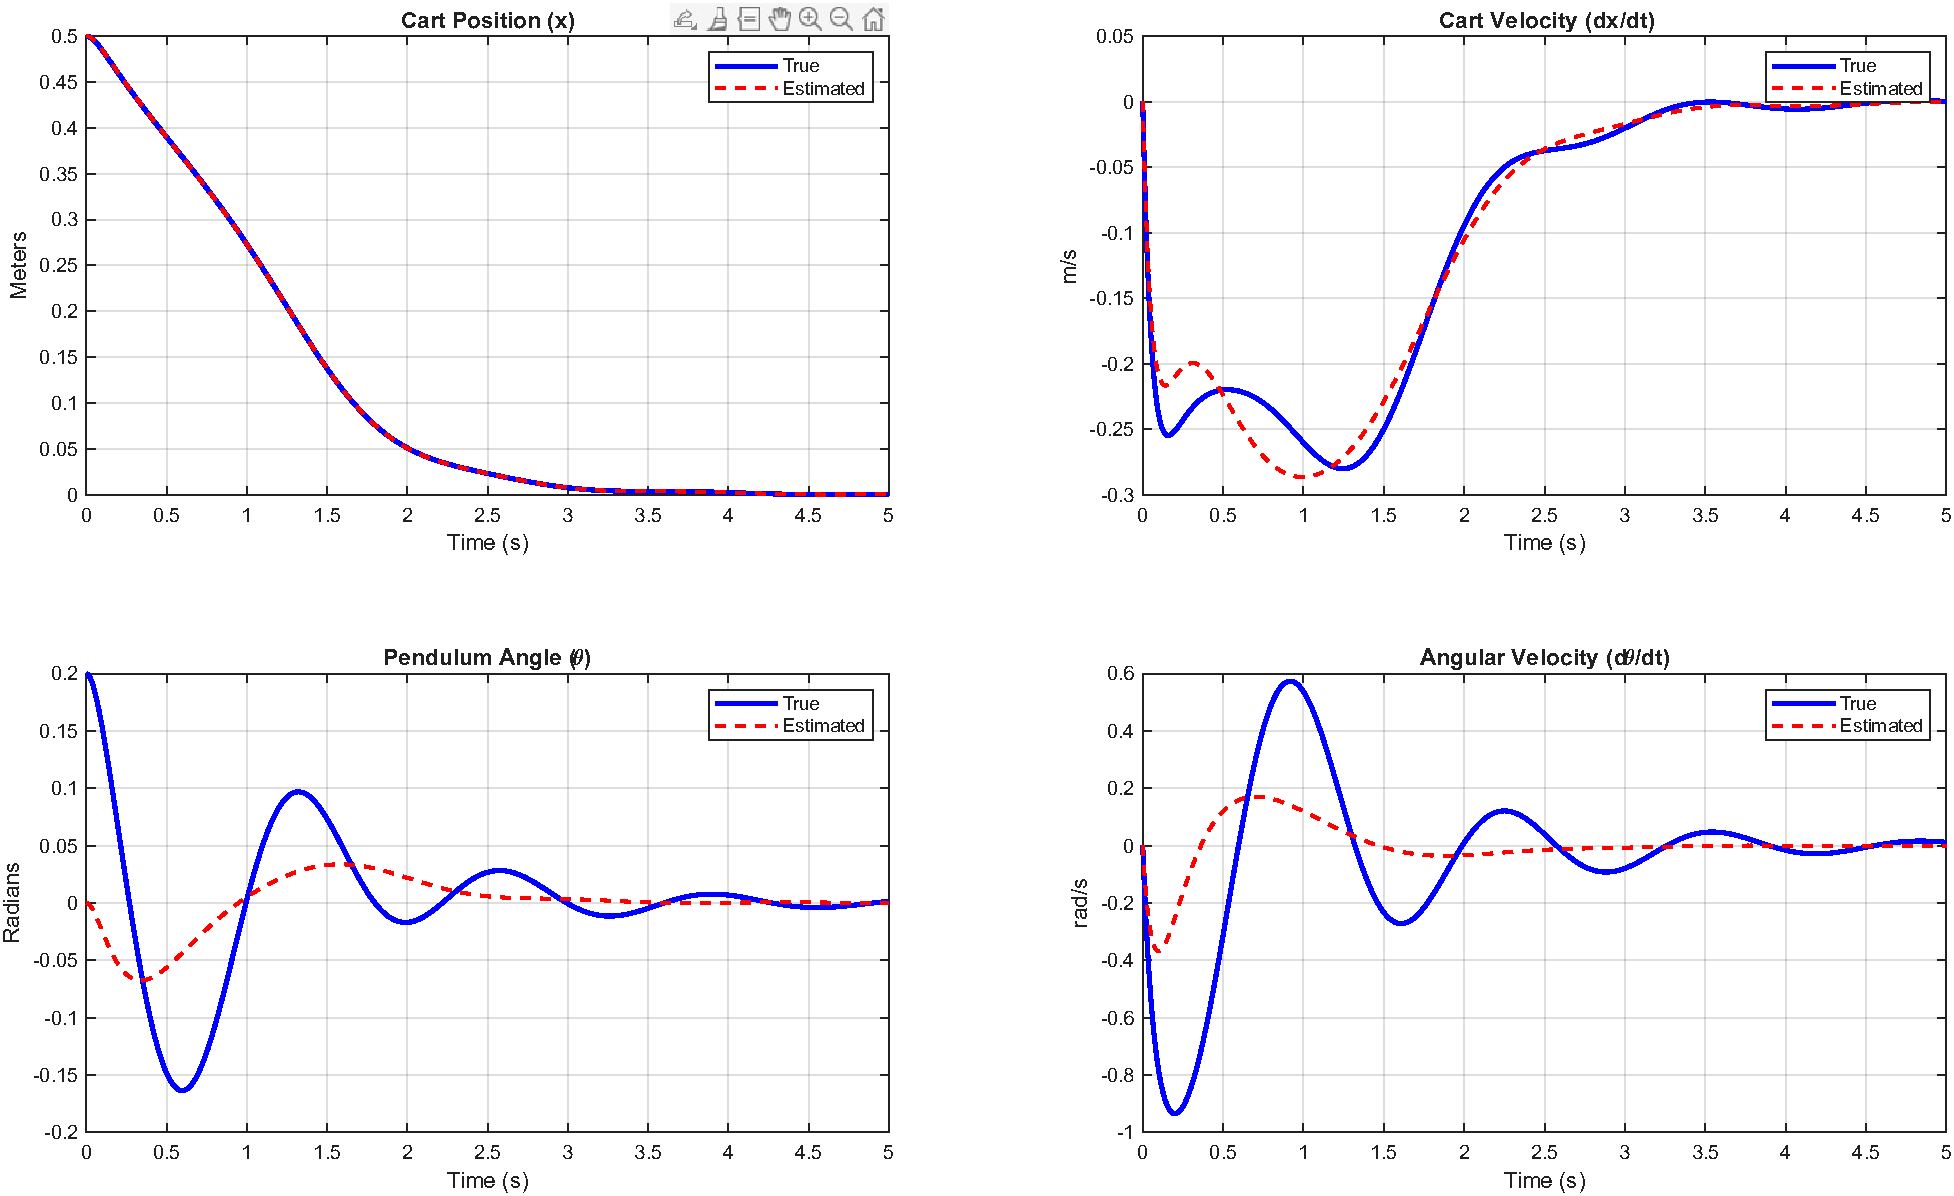
\includegraphics[width=0.9\textwidth]{./images/Kalman.pdf}
    \caption{مقایسه متغیرهای حالت واقعی سیستم (آبی) و مقادیر تخمین‌زده‌شده توسط فیلتر کالمن (قرمز)}
    \label{fig:kalman_estimation}
\end{figure}

همان‌طور که در شکل \ref{fig:kalman_estimation} مشاهده می‌شود، پس از رفع مشکل شرایط اولیه و تنظیم صحیح ماتریس $Q_k$، خطوط تخمینی در کسری از ثانیه و به نرمی بر روی مقادیر واقعی منطبق شده‌اند. به لطف این تخمین سریع و دقیق، کنترل‌کننده \lr{LQR} توانسته است نیروی صحیحی را اعمال کرده و نوسانات زاویه‌ای پاندول (که سنسوری برای آن وجود نداشت) را به طور کامل و با موفقیت میرا کند.

\section{پیاده‌سازی فیلتر کالمن در محیط سیمولینک و تحلیل اثر نویز سنسور}
\label{sec:kalman_simulink}

پس از طراحی و ارزیابی تئوریک کنترل‌کننده \lr{LQG} (ترکیب \lr{LQR} و فیلتر کالمن) در محیط اسکریپت متلب، گام بعدی پیاده‌سازی این ساختار بر روی مدل فیزیکی و غیرخطی سیستم در محیط سیمولینک است. هدف از این بخش، بررسی عملکرد مشاهده‌گر در شرایط واقع‌بینانه، به ویژه در حضور نویز اندازه‌گیری سنسور موقعیت ارابه می‌باشد.

\subsection{ساختار پیاده‌سازی در سیمولینک}

برای پیاده‌سازی فیلتر کالمن، بلوک‌های مشتق‌گیر ایده‌آل (که در بخش‌های قبل برای استخراج سرعت استفاده شده بودند) حذف گردیدند، زیرا این بلوک‌ها در برابر نویز به شدت ناپایدار عمل می‌کنند. به جای آن‌ها، یک بلوک فضای حالت (\lr{State-Space}) به عنوان «مشاهده‌گر» در حلقه کنترل قرار گرفت.

دینامیک این بلوک بر اساس معادله‌ی فیلتر کالمن $\dot{\hat{\mathbf{x}}} = (A - LC)\hat{\mathbf{x}} + Bu + Ly$ با ماتریس‌های زیر مقداردهی شد:
\begin{align*}
    A_{\mathrm{obs}} & = A - LC                              \\
    B_{\mathrm{obs}} & = \begin{bmatrix} B & L \end{bmatrix} \\
    C_{\mathrm{obs}} & = I_{4 \times 4}                      \\
    D_{\mathrm{obs}} & = 0_{4 \times 2}
\end{align*}

ورودی‌های این بلوک شامل نیروی کنترلی ($u$) و موقعیت اندازه‌گیری‌شده ارابه ($y$) است و خروجی آن، بردار حالت تخمینی ($\hat{\mathbf{x}}$) است که مستقیماً به ماتریس بهره کنترل‌کننده ($-K$) متصل می‌شود. شماتیک این پیاده‌سازی در شکل \ref{fig:kalman_simulink_model} نشان داده شده است.

\begin{figure}[ht!]
    \centering
    % دقت کنید که نام فایل عکس بلاک دیاگرام شما در اینجا قرار داده شده است
    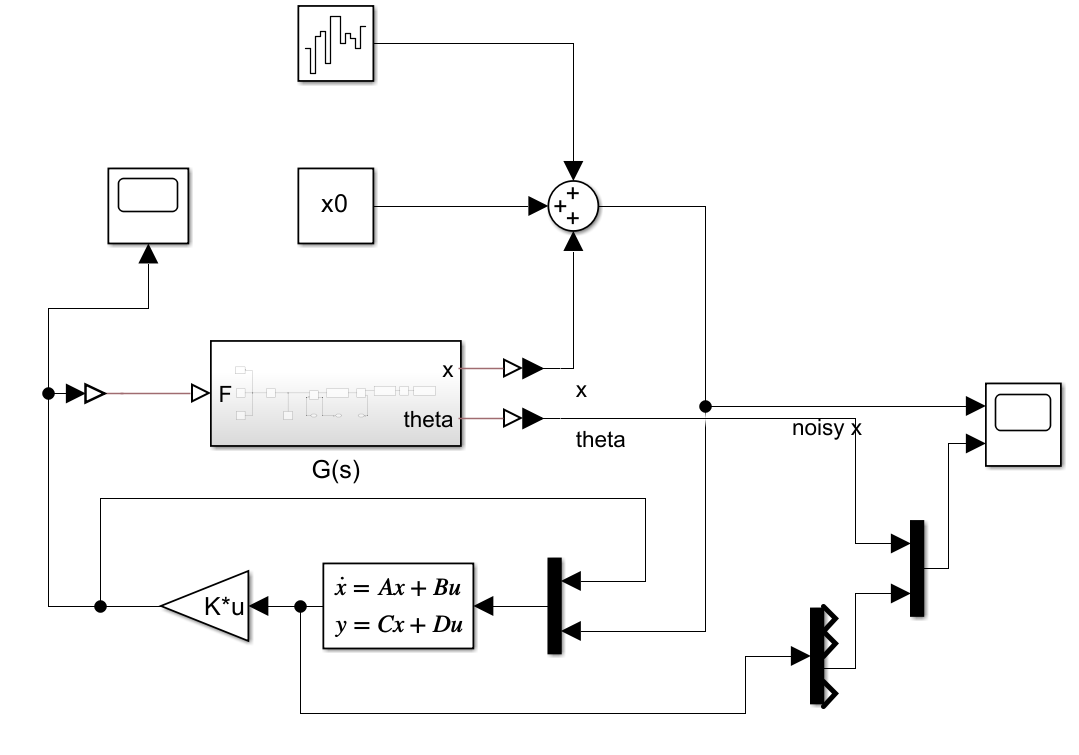
\includegraphics[width=0.9\textwidth]{./images/kalman_simulink.png}
    \caption{بلاک دیاگرام پیاده‌سازی سیستم \lr{LQG} با فیلتر کالمن و نویز سنسور در سیمولینک}
    \label{fig:kalman_simulink_model}
\end{figure}

نکته‌ی حیاتی در این پیاده‌سازی، تطابق شرایط اولیه‌ی مشاهده‌گر با واقعیت فیزیکی است. از آنجا که ارابه حرکت خود را از موقعیت $x_0 = 0.5~\mathrm{m}$ آغاز می‌کند، مقدار اولیه‌ی بلوک فضای حالتِ فیلتر کالمن نیز روی بردار $[0.5, 0, 0, 0]^T$ تنظیم شد تا از بروز خطای تخمین ناگهانی (پرش) در لحظه‌ی راه‌اندازی جلوگیری شود.

\subsection{چالش نویز سنسور و پدیده‌ی لرزش (\lr{Chattering})}

در دنیای واقعی، سنسورهای موقعیت (مانند انکودرها) همواره دارای نویز فرکانس‌بالا هستند. برای شبیه‌سازی این شرایط، از بلوک \lr{Band-Limited White Noise} استفاده شد و نویز مستقیماً به خروجی موقعیت ارابه ($x$) اضافه گردید.

در شبیه‌سازی‌های اولیه با نویز، مشاهده شد که سیستم در حالت ماندگار (\lr{Steady-State}) دچار لرزش پیوسته و نوسانات ریز در زاویه‌ی آونگ می‌شود. تحلیل این رفتار نشان داد که دو عامل اصلی در بروز این پدیده نقش داشته‌اند:
\begin{enumerate}
    \item \textbf{ماهیت پله‌ای نویز در شبیه‌سازی دیجیتال:} بزرگ بودن زمان نمونه‌برداری (\lr{Sample Time}) بلوک نویز باعث می‌شد سیگنال به صورت پله‌ای تغییر کند. فیلتر کالمن این پرش‌های پله‌ای را به عنوان سرعت‌های لحظه‌ایِ بسیار بزرگ تفسیر کرده و به کنترل‌کننده فرمان‌های نوسانی و شدیدی ارسال می‌کرد. با کاهش زمان نمونه‌برداری به $0.001$ ثانیه، نویز به یک سیگنال پیوسته و واقع‌بینانه‌تر تبدیل شد.
    \item \textbf{تنظیم بیش از حد تهاجمیِ فیلتر:} مقادیر بزرگ ماتریس کوواریانس نویز فرآیند ($Q_k$) سبب می‌شد فیلتر کالمن به جای اعتماد به مدل فیزیکی نرم سیستم، تغییرات نویزی سنسور را به شدت دنبال کند.
\end{enumerate}

برای رفع این مشکل، ماتریس‌های فیلتر کالمن با رویکرد «اعتماد بیشتر به فیزیک سیستم و دفع نویز فرکانس‌بالا» به صورت زیر بازتنظیم شدند:
\begin{equation}
    Q_k = \mathrm{diag}(0.1, 0.01, 0.1, 1) \quad , \quad R_k = 0.001
\end{equation}

\subsection{نتایج شبیه‌سازی نهایی}

با اعمال اصلاحات فوق، شبیه‌سازی سیستم \lr{LQG} در حضور نویز اندازه‌گیری مجدداً اجرا گردید. شکل \ref{fig:kalman_simulink_results} پاسخ زمانی سیستم را تحت این شرایط نشان می‌دهد.

\begin{figure}[ht!]
    \centering
    % نام فایل خروجی اسکوپ که ارسال کردید. دقت کنید که نام فایل بدون حرف n تایپ شده بود.
    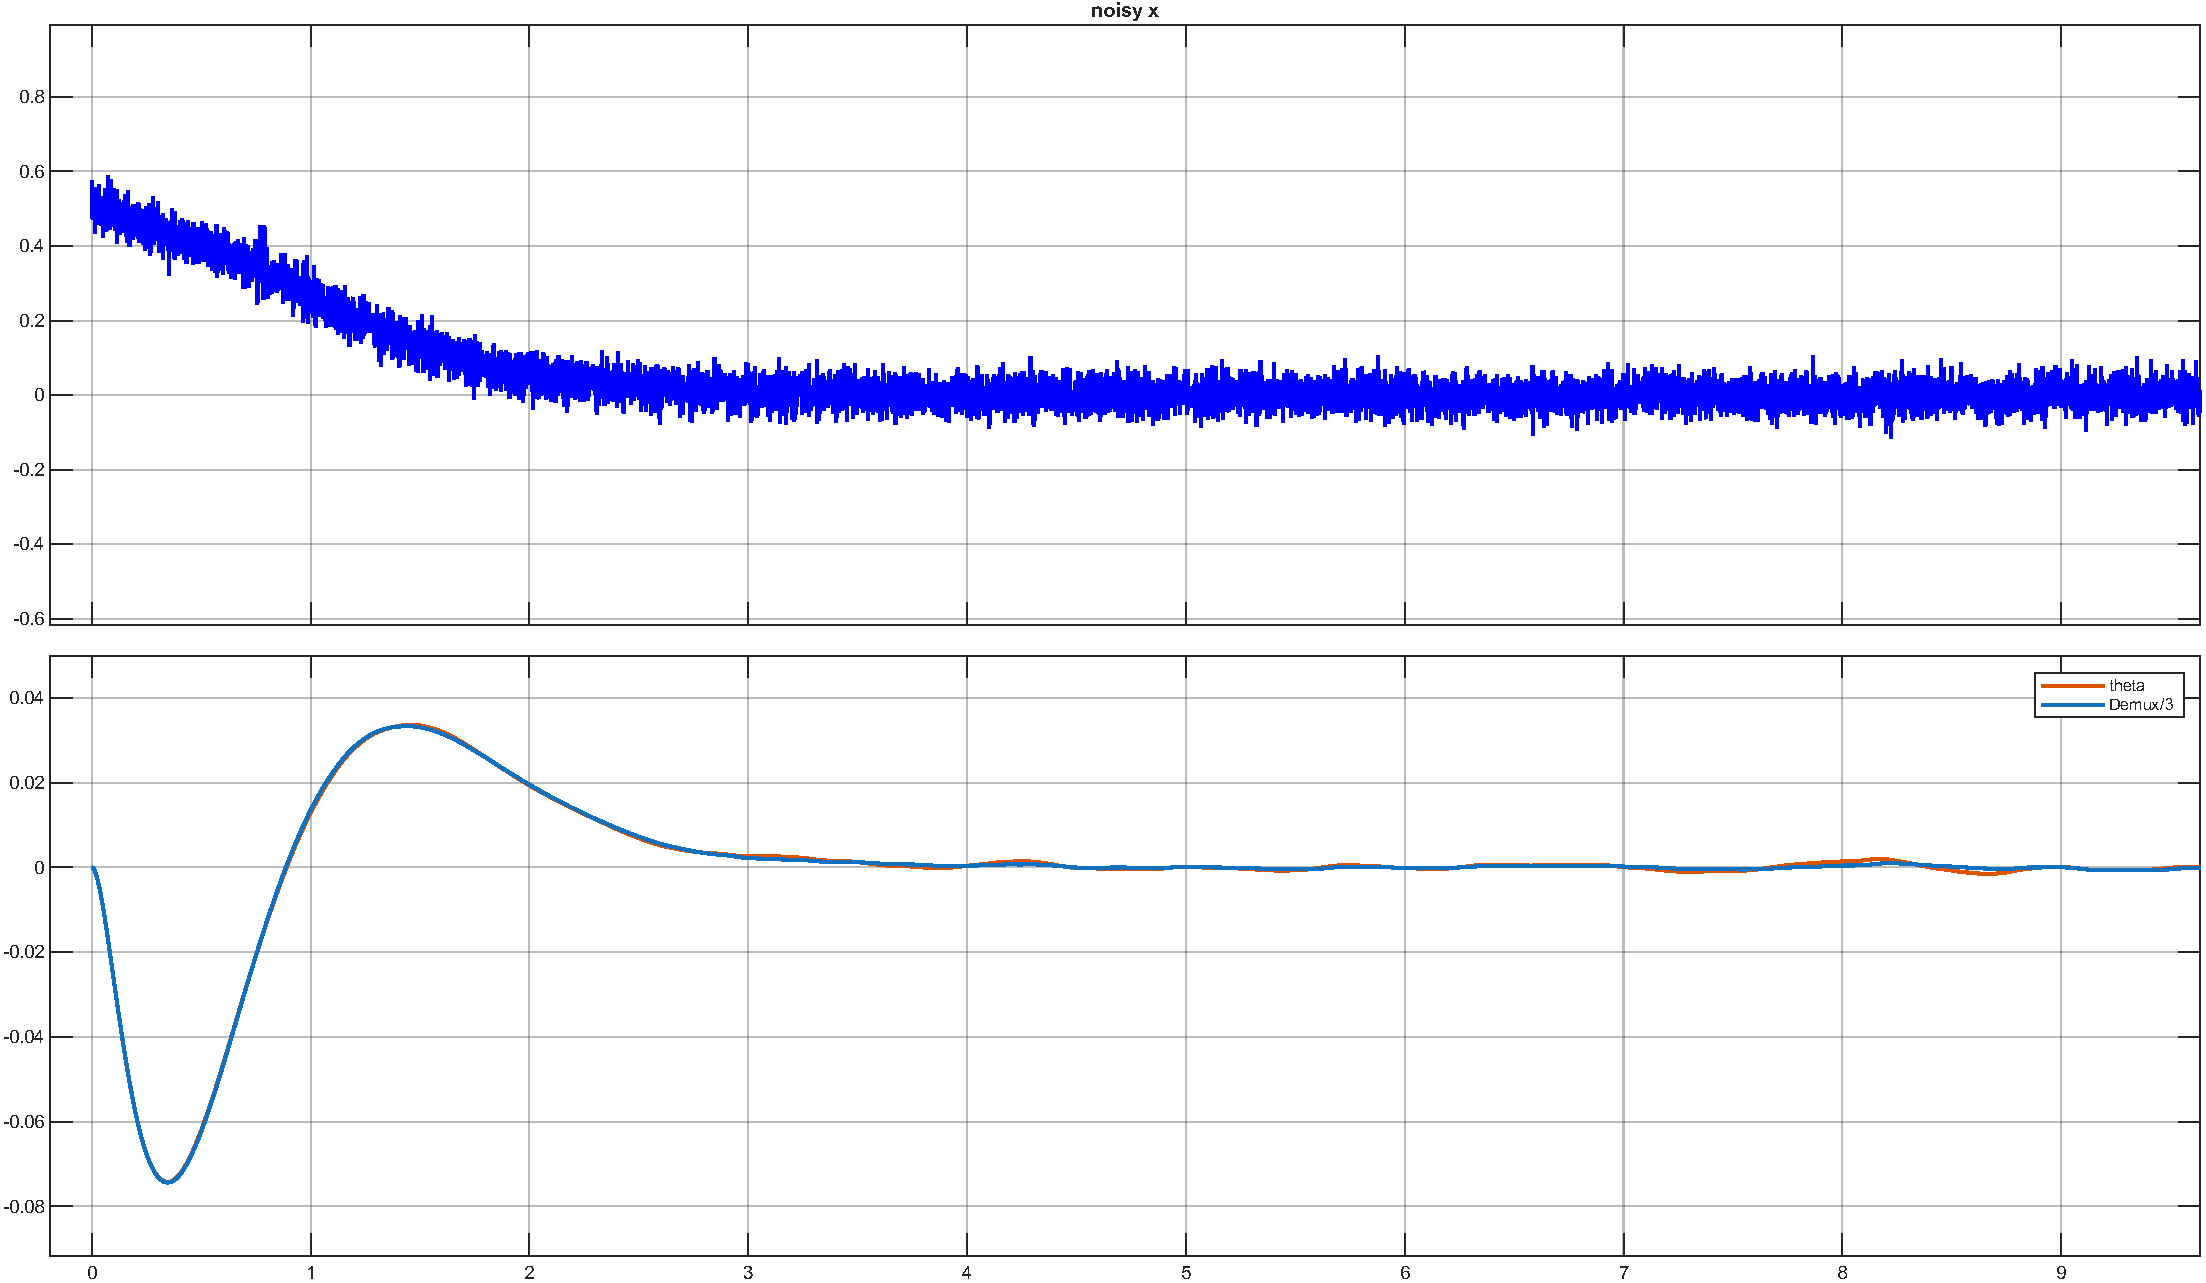
\includegraphics[width=\textwidth]{./images/kalman_simulink.pdf}
    \caption{پاسخ زمانی سیستم در حضور نویز؛ نمودار بالا: سیگنال نویزی سنسور ارابه ($x$)، نمودار پایین: همگرایی زاویه واقعی ($\theta$) و زاویه تخمینی آونگ.}
    \label{fig:kalman_simulink_results}
\end{figure}

همان‌طور که در نمودار بالای شکل \ref{fig:kalman_simulink_results} مشخص است، سیگنال اندازه‌گیری‌شده توسط سنسور دارای نویز پیوسته و شدیدی است. با این وجود، فیلتر کالمن به خوبی توانسته است این نویز را فیلتر کرده و دینامیک پنهان سیستم را استخراج کند. نمودار پایین نشان می‌دهد که متغیر حالت زاویه آونگ ($\theta$) که اصلاً اندازه‌گیری نشده است، توسط فیلتر به درستی تخمین زده شده (خط آبی‌رنگ) و کاملاً بر رفتار واقعی آونگ منطبق است.

همچنین، به دلیل تنظیم صحیح و نرم‌تر پارامترهای $Q_k$، پدیده‌ی لرزش به طور کامل برطرف شده و موتور از اعمال ضربات متوالی بازداشته شده است؛ در نتیجه، آونگ پس از فاز گذرا، بدون هیچ‌گونه نوسان ماندگاری به حالت سکون و تعادل کامل (صفر) دست یافته است.

\section{کد متلب مدل‌سازی فضای‌حالت سیستم آونگ--ارابه}
\label{app:ss_modeling_code}

در این ضمیمه، اسکریپت متلب \lr{ss\_modeling.m} که برای مدل‌سازی فضای‌حالت سیستم آونگ--ارابه استفاده شده است، آورده می‌شود.

\begin{LTRlisting}
    \lstinputlisting[
        style=matlabStyle,
        caption={\texttt{ss\_modeling.m}},
        label={lst:ss_modeling}
    ]{./scripts/ss_modeling.m}
\end{LTRlisting}

\section{کد متلب طراحی کنترل‌کننده \lr{LQR}}
\label{app:lqr_code}

در این ضمیمه، اسکریپت متلب \lr{LQR.m} که برای محاسبه ماتریس بهره بهینه، اعمال قانون فیدبک حالت و رسم پاسخ‌های زمانی سیستم استفاده شده است، آورده می‌شود.

\begin{LTRlisting}
    \lstinputlisting[
        style=matlabStyle,
        caption={\texttt{LQR.m}},
        label={lst:lqr_code}
    ]{./scripts/LQR.m}
\end{LTRlisting}

\section{کد متلب طراحی فیلتر کالمن (\lr{LQG})}
\label{app:kalman_code}

\begin{LTRlisting}
    \lstinputlisting[
        style=matlabStyle,
        caption={\texttt{kalman.m}},
        label={lst:kalman_code}
    ]{./scripts/kalman.m}
\end{LTRlisting}

\end{document}
